%!TEX program = lualatex
\documentclass[10pt,a4paper,sans,colorlinks]{moderncv}
\title{Certificates}
%%%%%%%%%%%%%%%%%%%%%%%%%%%%%%%%%%%%%%%%
%%%%%%%%%%%%%%%%%%%%%%%%%%%%%%%%%%%%%%%%
\def\markdownRendererLink#1#2#3#4{\href{#3}{#1}{}{}} % fix markdown link
\usepackage{blindtext} % blind text
\usepackage{tabularx} % flexible column X
\usepackage{booktabs} % \toprule, \midrule, \bottomrule
\usepackage{listings} % code listing
\usepackage{subcaption} % subfigures
\usepackage{ragged2e} % \justify
\usepackage{graphicx} % includegraphics
\usepackage{acronym} % \newacro and \ac
\graphicspath{{figs}} % includegraphics figs
\usepackage{url} % \url
\usepackage{array}
\newcommand{\ie}[0]{\textit{i.e.},~}
\newcommand{\eg}[0]{\textit{e.g.},~}
\newcommand{\etal}[0]{\textit{et al.}~}
\newcommand\setEnumItemNoSep{% called preamble
    \usepackage{enumitem}
    \setlist[itemize]{noitemsep, nosep, topsep=0pt, partopsep=0pt, parsep=0pt, itemsep=0pt, leftmargin=*,rightmargin=0pt} % set enum key
    \setlist[enumerate]{noitemsep, nosep, topsep=0pt, partopsep=0pt, parsep=0pt, itemsep=0pt, leftmargin=*,rightmargin=0pt} % set enum key
}
\newcommand\setItemizeUseHyphen{% called preamble
    \usepackage{enumitem}
    \def\labelitemi{-}
}
\newcommand\setLargeGeometry{% called in preamble
    \usepackage[a4paper, left=20mm, top=20mm]{geometry}
}
\newcommand\setParagraphReducedSpacing{% called preamble
    \linespread{1}
    \setlength{\parskip}{0pt}
    \setlength{\parsep}{0pt}
}
\newcommand{\gingaITU}{\href{https://www.itu.int/rec/T-REC-H.761}{TV API standards}}
\newcommand{\gingaSBTVD}{\href{https://forumsbtvd.org.br/legislacao-e-normas-tecnicas/normas-tecnicas-da-tv-digital/english/}{TV API standards}}

%%%%%%%%%%%%%%%%%%%%%%%%%%%%%%%%%%%%%%%%
% -- alan config end
%%%%%%%%%%%%%%%%%%%%%%%%%%%%%%%%%%%%%%%%

%%%%%%%%%%%%%%%%%%%%%%%%%%%%%%%%%%%%%%%%
% -- alan moderncv begin
%%%%%%%%%%%%%%%%%%%%%%%%%%%%%%%%%%%%%%%%
\usepackage{footmisc} % enabling footnotes for moderncv
\moderncvstyle{banking}
\moderncvcolor{blue}
\name{Tousif}{Hasan}
\email{thlavlu@gmail.com}
\homepage{thlavlu@github.io}
\collectionadd[github]{socials}{\protect\httpslink[github]{github.com/thlavlu}}
\collectionadd[googlescholar]{socials}{\protect\httpslink[scholar]{scholar.google.com/citations?hl=en&user=1bEOmkUAAAAJ&sortby=pubdate}}

% modercv has no figure, table
\usepackage{float}
\newfloat{figure}{htbp}{figs}
\newfloat{table}{htbp}{figs}
\newcommand\setHyperrefBlueLinks{% called inside document
    \definecolor{links}{HTML}{2A1B81}
    \hypersetup{
        urlcolor=links,
        linkcolor=links,
        citecolor=links
    }
}
%%%%%%%%%%%%%%%%%%%%%%%%%%%%%%%%%%%%%%%%
                 THL
%%%%%%%%%%%%%%%%%%%%%%%%%%%%%%%%%%%%%%%%

\setLargeGeometry
\setParagraphReducedSpacing
\usepackage{graphbox}
\usepackage{tabularx}
\usepackage{graphicx}
\usepackage{pgffor}
\usepackage{pgfkeys, pgfcalendar}
\usepackage{float}
\usepackage{multicol}

% moderncv Table of Contents
% based on https://tex.stackexchange.com/questions/158803/add-a-table-of-contents-into-a-moderncv-document
\makeatletter
\newcommand\@pnumwidth{1.55em}
\newcommand\@tocrmarg{2.55em}
\newcommand\@dotsep{4.5}
\makeatother
\usepackage{titletoc}
\makeatletter
\setlength\columnsep{20pt}
\setcounter{tocdepth}{0}
\newcommand\contentsname{Table of Contents}
\newcommand\tableofcontents{%
\addtocontents{toc}{\protect\setcounter{tocdepth}{0}}
\section*{\contentsname}
\addtocontents{toc}{\protect\setcounter{tocdepth}{2}}\@starttoc{toc}}
\usepackage{titletoc}
\titlecontents*{section}[0pt]{}{}{\textbullet}{\ \thecontentspage}[\\][]
\titlecontents{section}[0pt]{}{}{}{\leaders\hbox{\normalfont$\m@th\mkern \@dotsep mu\hbox{.}\mkern \@dotsep mu$}\hfill\normalsize\thecontentspage}[]
\makeatother
% moderncv Table of Contents

%%%%%%%%%%%%%%%%%%%%%%%%%%%%%%%%%%%%%%%%
% document
%%%%%%%%%%%%%%%%%%%%%%%%%%%%%%%%%%%%%%%%
\begin{document}
\setHyperrefBlueLinks
\makecvtitle
\tableofcontents

%%%%%%%%%%%%%%%%%%%%%%%%%%%%%%%%%%%%%%%%
% UFPB B.Sc. certificates
%%%%%%%%%%%%%%%%%%%%%%%%%%%%%%%%%%%%%%%%
\newpage
\section{UFPB B.Sc. certificates}
The next figure presents my B.Sc. certificate in Portuguese.
It says a B.Sc. in Computer Science degree from the Federal University of Paraiba, Brazil.

\begin{figure}
    \centering
    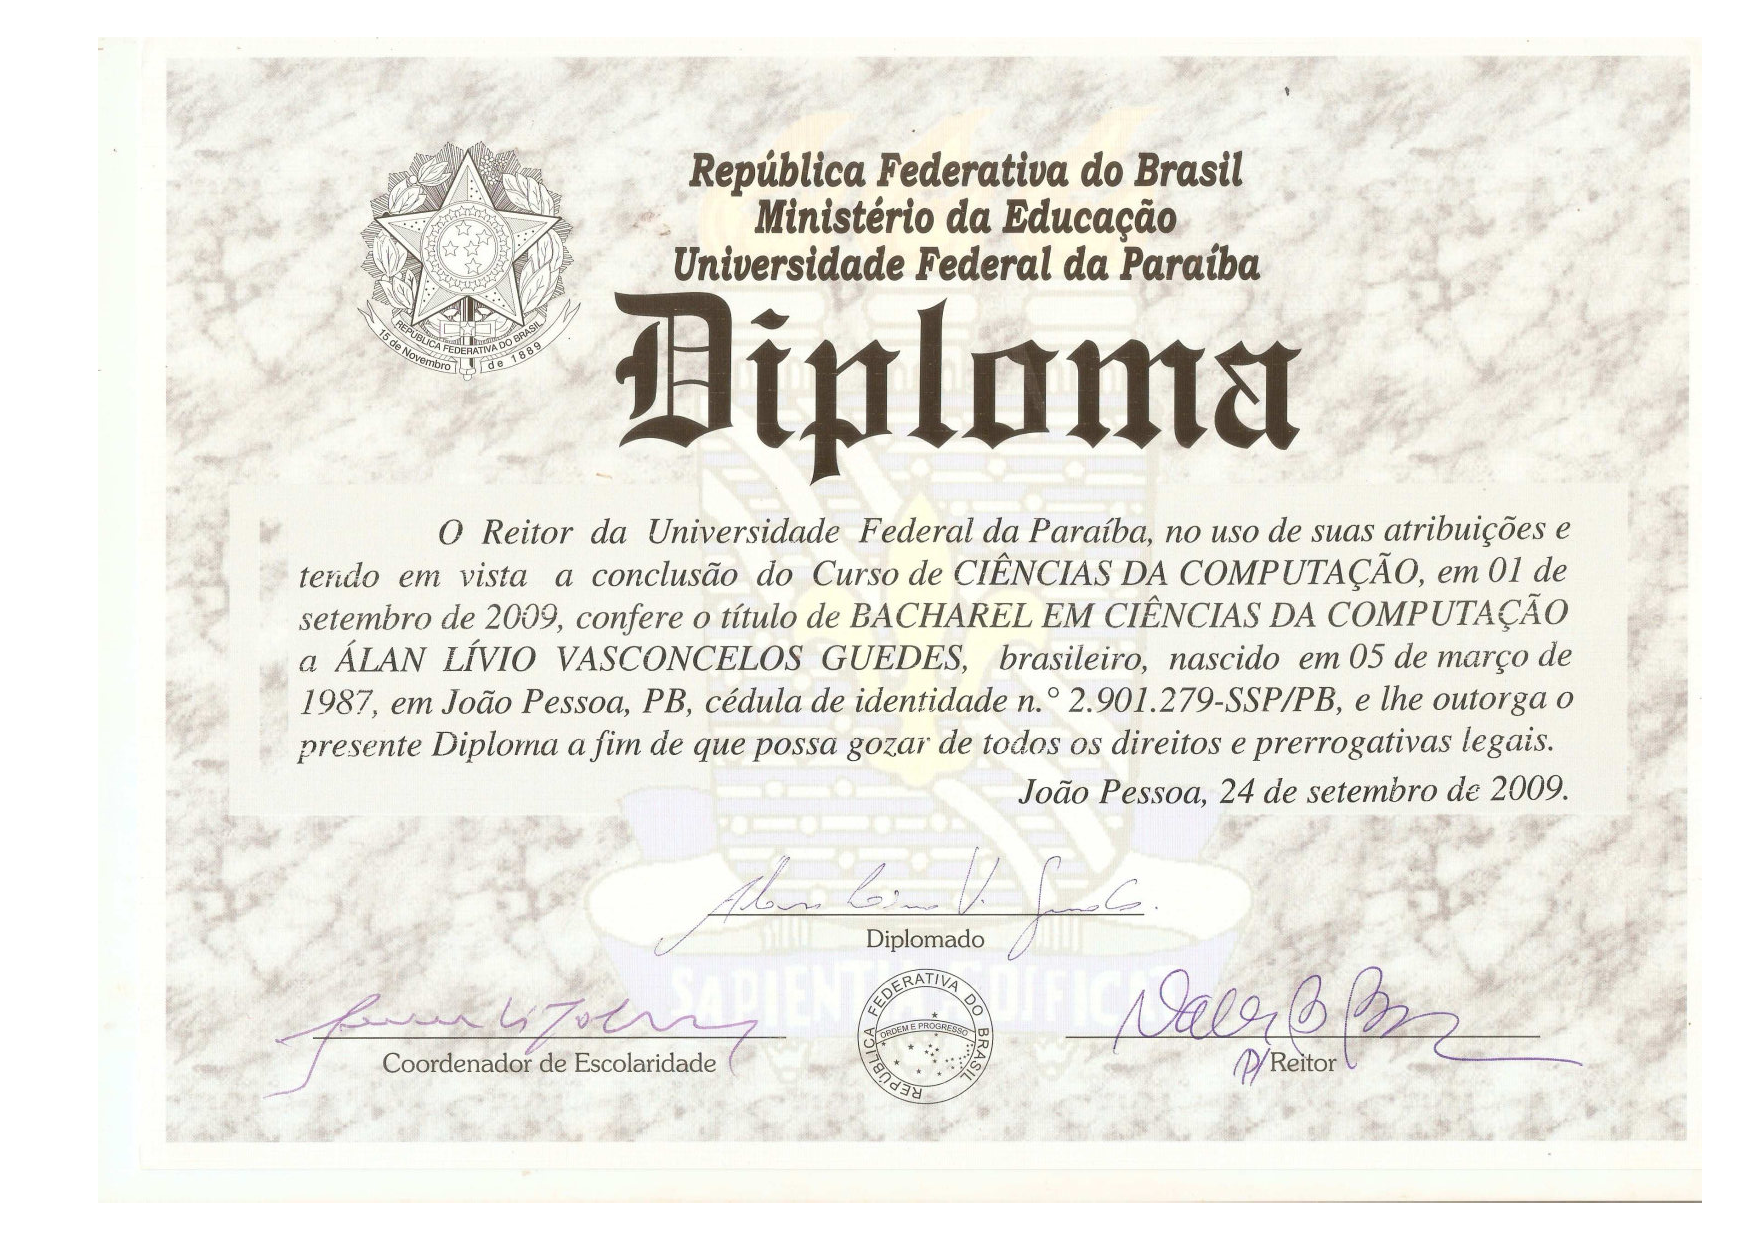
\includegraphics[align=t,width=\textwidth,height=0.3\paperheight, keepaspectratio=true]{certificates/bsc-certificate.pdf}
\end{figure}

\newpage

The next figure presents the first part of the grades of my B.Sc. in Portuguese.
It informs done with a general score (CRA in Portuguese) of \textbf{7.72}.
It includes three Physics and three Differential Calculus courses.
From computer science fundaments, it includes two Data Structures courses, Logic and Design \& Analyses of Algorithms. In particular, I archive the max degree 10.
\vspace{2em}
\begin{figure}
    \centering
    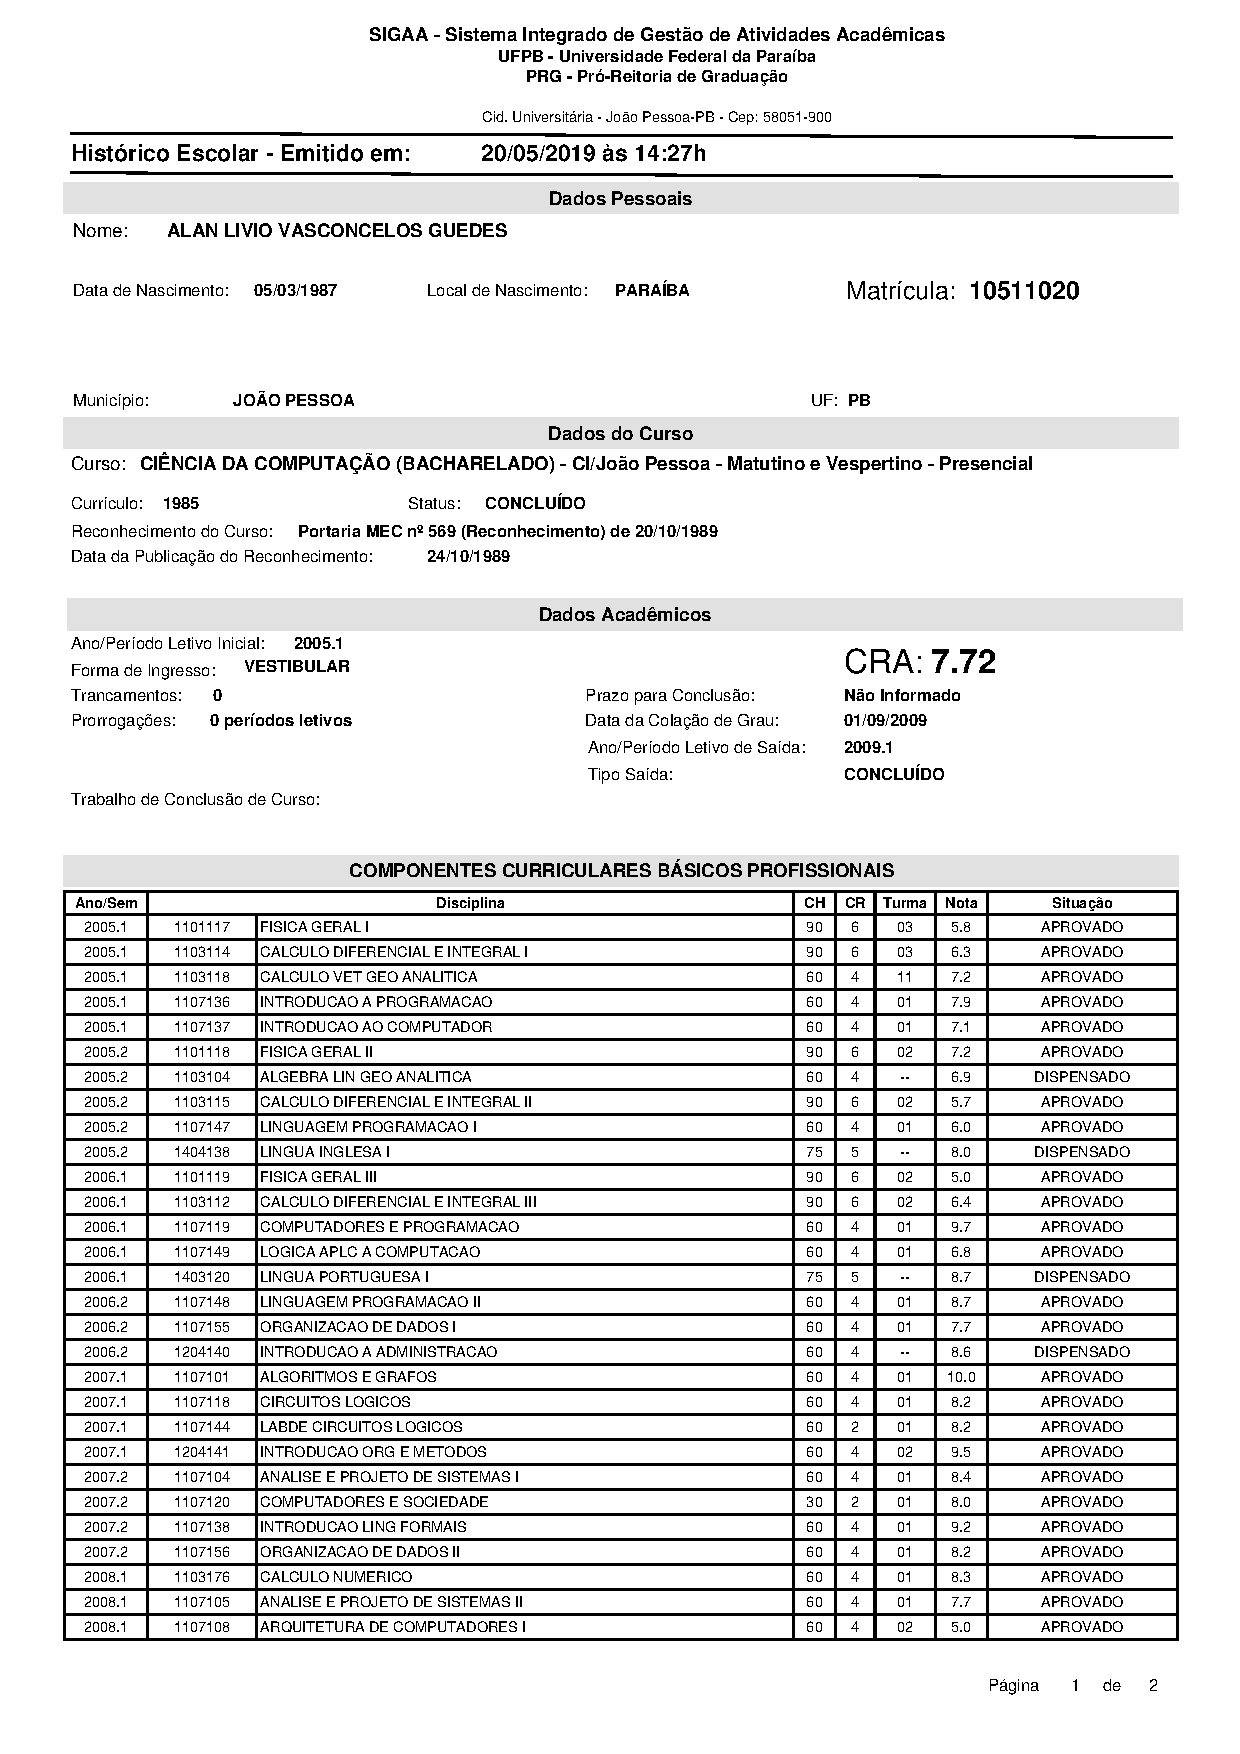
\includegraphics[align=t,width=\textwidth,height=0.6\paperheight, keepaspectratio=true, trim=0cm 0cm 0cm 2cm]{certificates/bsc-grades.pdf}
\end{figure}

\newpage

The next figure presents the second part of the grades of my B.Sc. in Portuguese.
The courses include Data Bases, Software Engineering, Computer Networks, and Compilers.
While extra courses include Psychology, Multimedia Systems, and Economics.
It shows a total of 2895 hours.
\vspace{2em}
\begin{figure}
    \centering
    \includegraphics[align=t,width=\textwidth,height=0.6\paperheight, keepaspectratio=true,page=2]{certificates/bsc-grades.pdf}
\end{figure}

\newpage

%%%%%%%%%%%%%%%%%%%%%%%%%%%%%%%%%%%%%%%%
% UFPB M.Sc. certificates
%%%%%%%%%%%%%%%%%%%%%%%%%%%%%%%%%%%%%%%%
\section{UFPB  M.Sc. certificates}

The next figure presents my M.Sc. certificate in Portuguese.
It informs an M.Sc. degree in Informatics from the Federal University of Paraíba, Brazil.

\begin{figure}
    \centering
    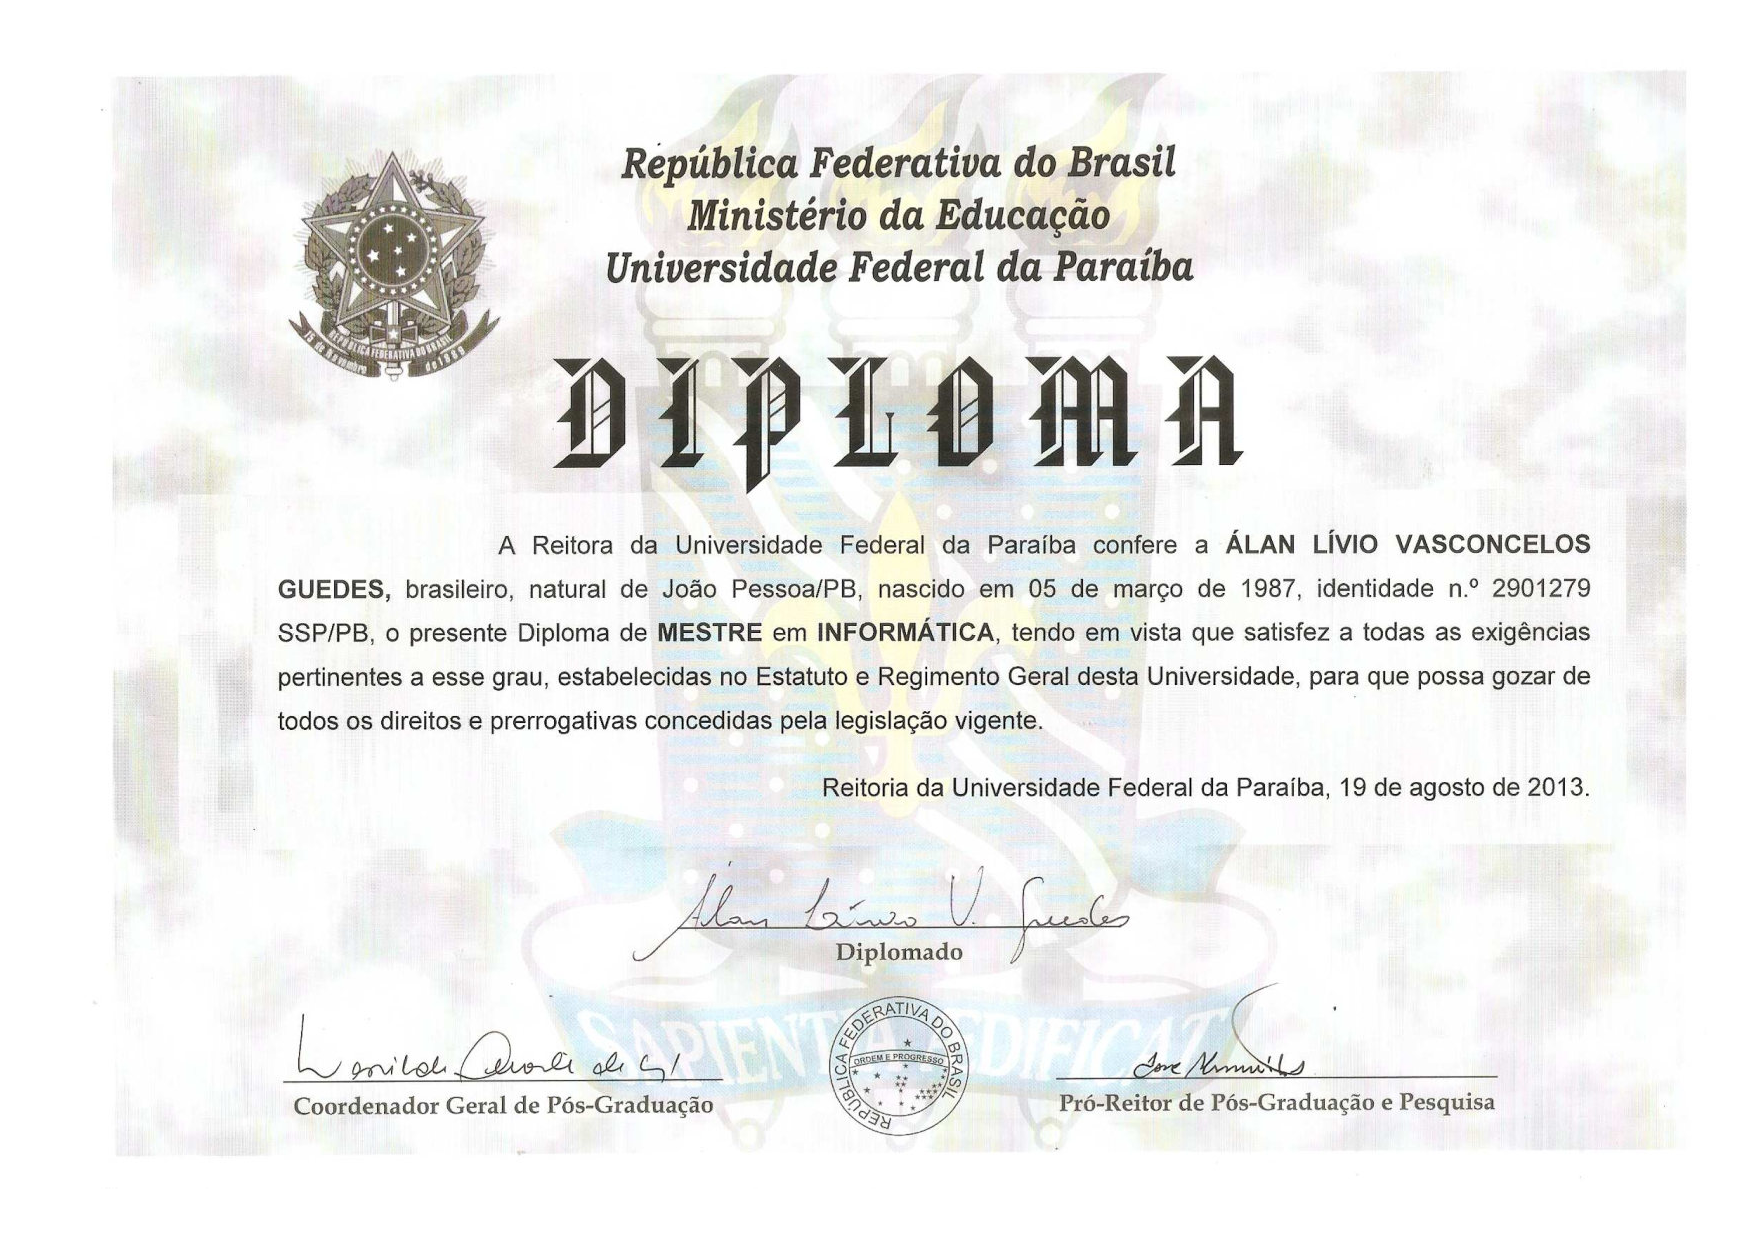
\includegraphics[align=t,width=\textwidth,height=0.3\paperheight, keepaspectratio=true]{certificates/msc-certificate.pdf}
\end{figure}

\newpage
The next figure presents the first part of my M.Sc. in Portuguese grades.
It informs done with a general score (CRA in Portuguese) of \textbf{8.12}.
The courses include Analyses of Algorithms, Computer Architecture, and Computing Theory.
The extra courses include Distributed Systems and Multimedia Systems.
\vspace{1em}
\begin{figure}
    \centering
    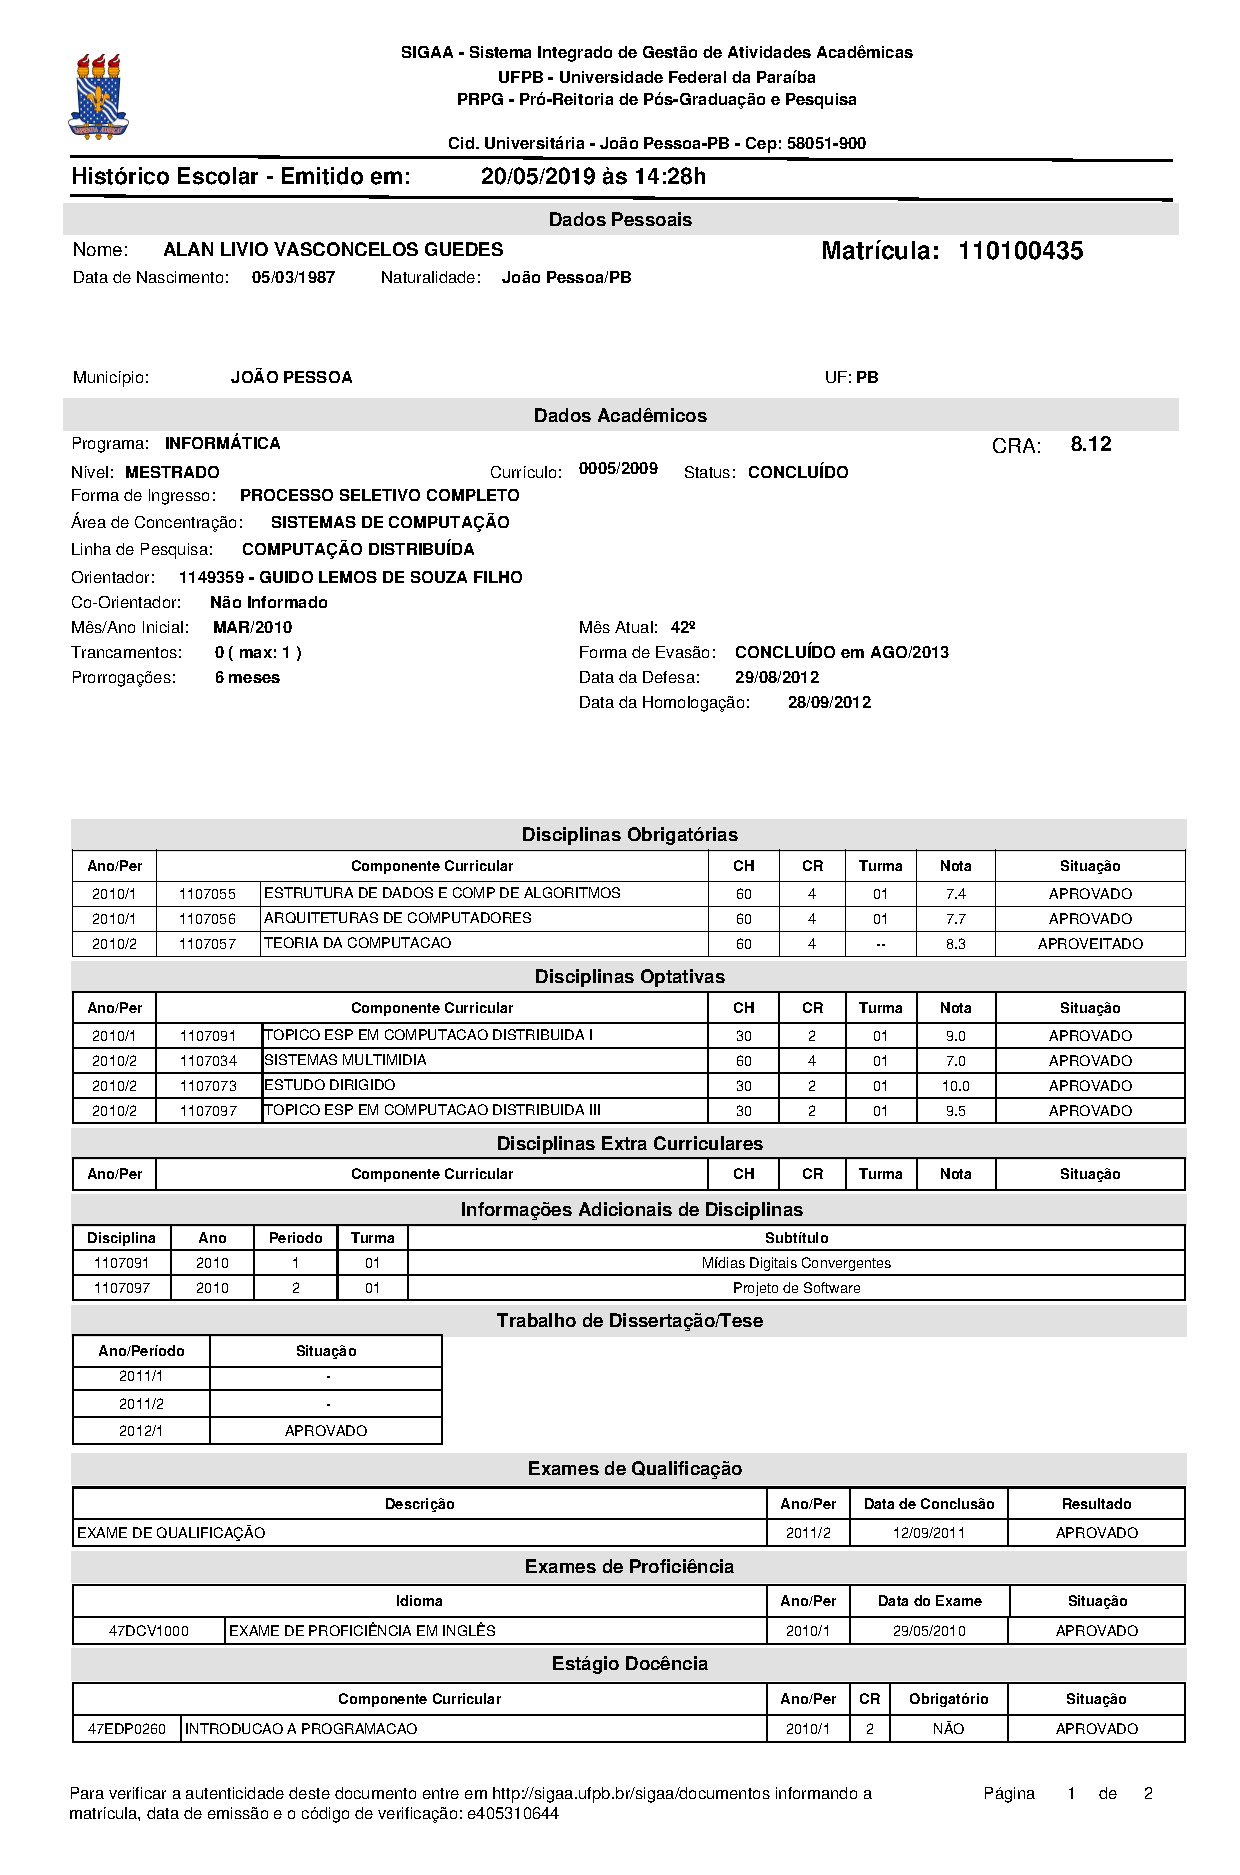
\includegraphics[align=t,width=\textwidth,height=0.6\paperheight, keepaspectratio=true, trim=0cm 0cm 0cm 2cm]{certificates/msc-grades.pdf}
\end{figure}

\newpage
The next figure presents the second part of the grades of my B.Sc. in Portuguese.
It informs the Master Thesis named \href{https://repositorio.ufpb.br/jspui/handle/tede/6087}{A Solution for Running Ginga-NCL Applications Using Second Screen on BroadBandTV Systems}.
\vspace{1em}
\begin{figure}
    \centering
    \includegraphics[align=t,width=\textwidth,height=0.6\paperheight, keepaspectratio=true, page=2, trim=0cm 0cm 0cm 2cm]{certificates/msc-grades.pdf}
\end{figure}


%%%%%%%%%%%%%%%%%%%%%%%%%%%%%%%%%%%%%%%%
% PUC-Rio Ph.D. certificates
%%%%%%%%%%%%%%%%%%%%%%%%%%%%%%%%%%%%%%%%
\newpage
\section{PUC-Rio Ph.D. certificates}

The next figure presents my Ph.D. certificate in Portuguese.
It says: "The dean of Pontifical Catholically University of Rio de Janeiro, in his attributions and given that was fulfilled with all legal requirements, as well the university requirements, grants to: Alan Livio Vasconcelos Guedes, the degree of Doctor in Science - Informatics with all the prerogatives, rights, and honors."
The bottom part contains signatures from the director of the "Admission and Registry" department and the dean.

\begin{figure}
    \centering
    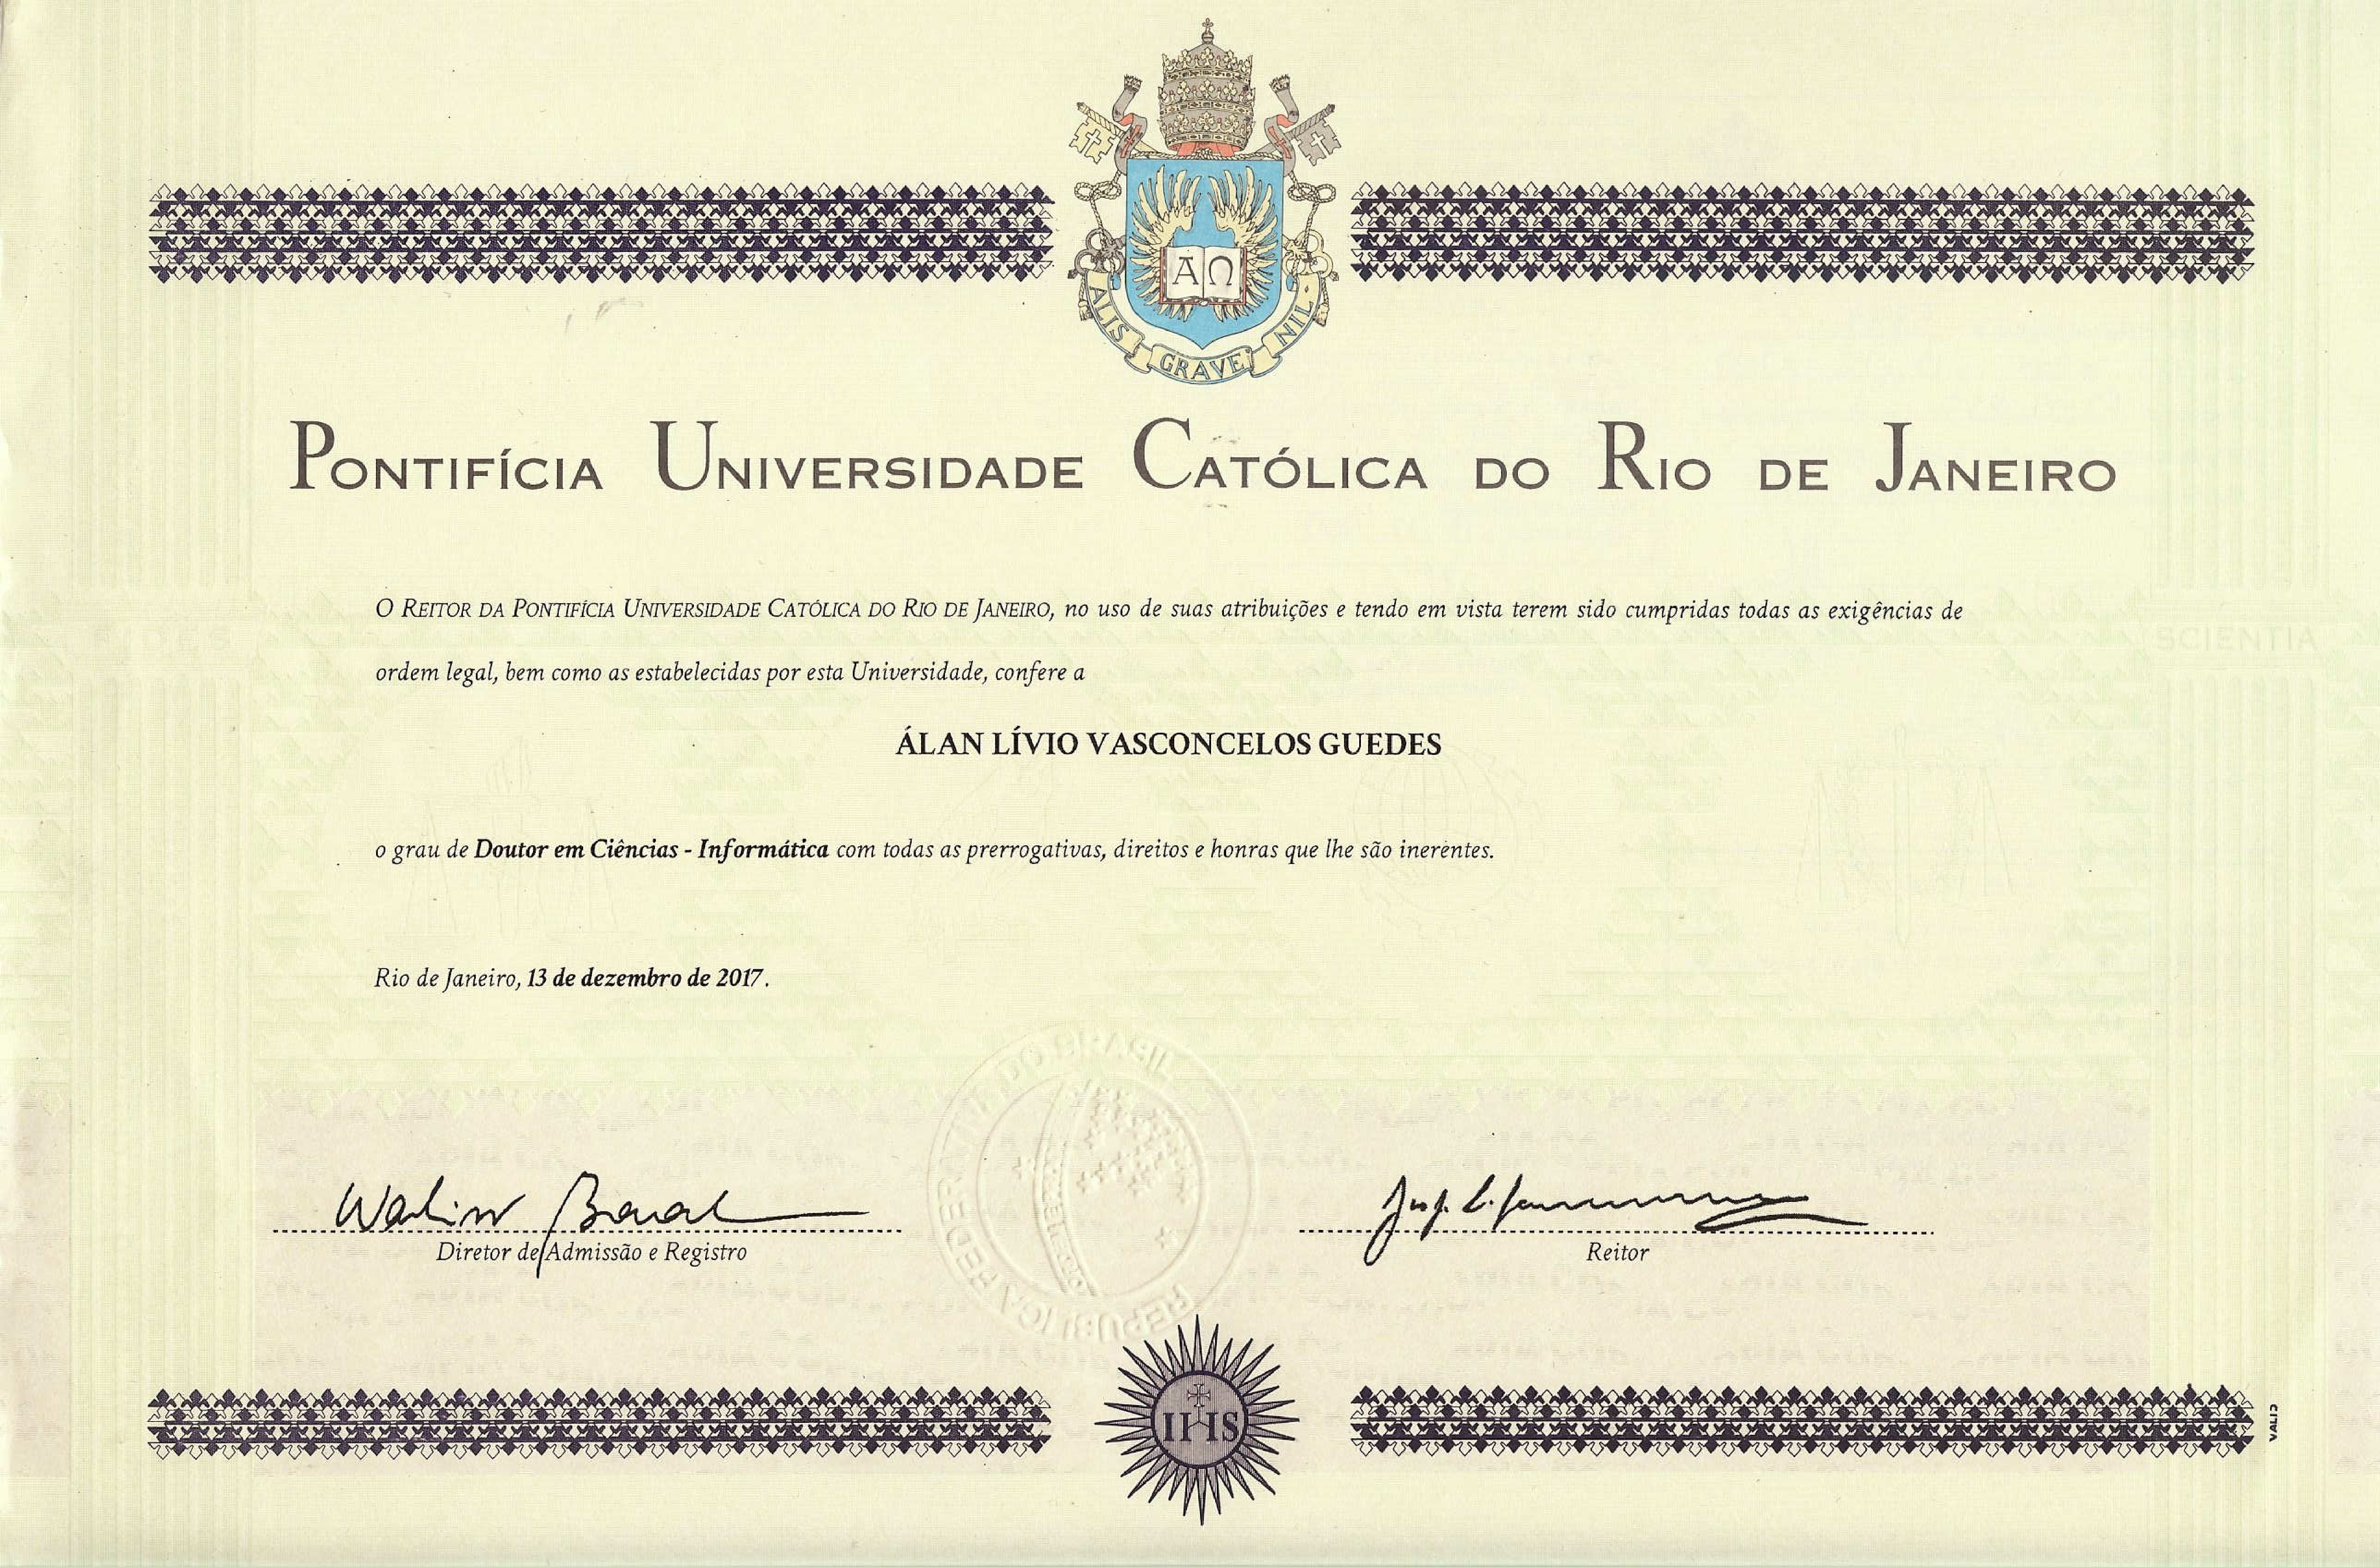
\includegraphics[align=t,width=\textwidth,height=0.3\paperheight, keepaspectratio=true]{certificates/phd-certificate.pdf}
\end{figure}

\newpage
The next figure presents the first page of grades from my Ph.D. in Portuguese.
It informs done with a general score ("Coeficiente de Rendimento" in Portuguese) of \textbf{8.5}.
It includes courses in Computer Graphics, Mobile Computing, and Multimedia Systems.

\begin{figure}
    \centering
    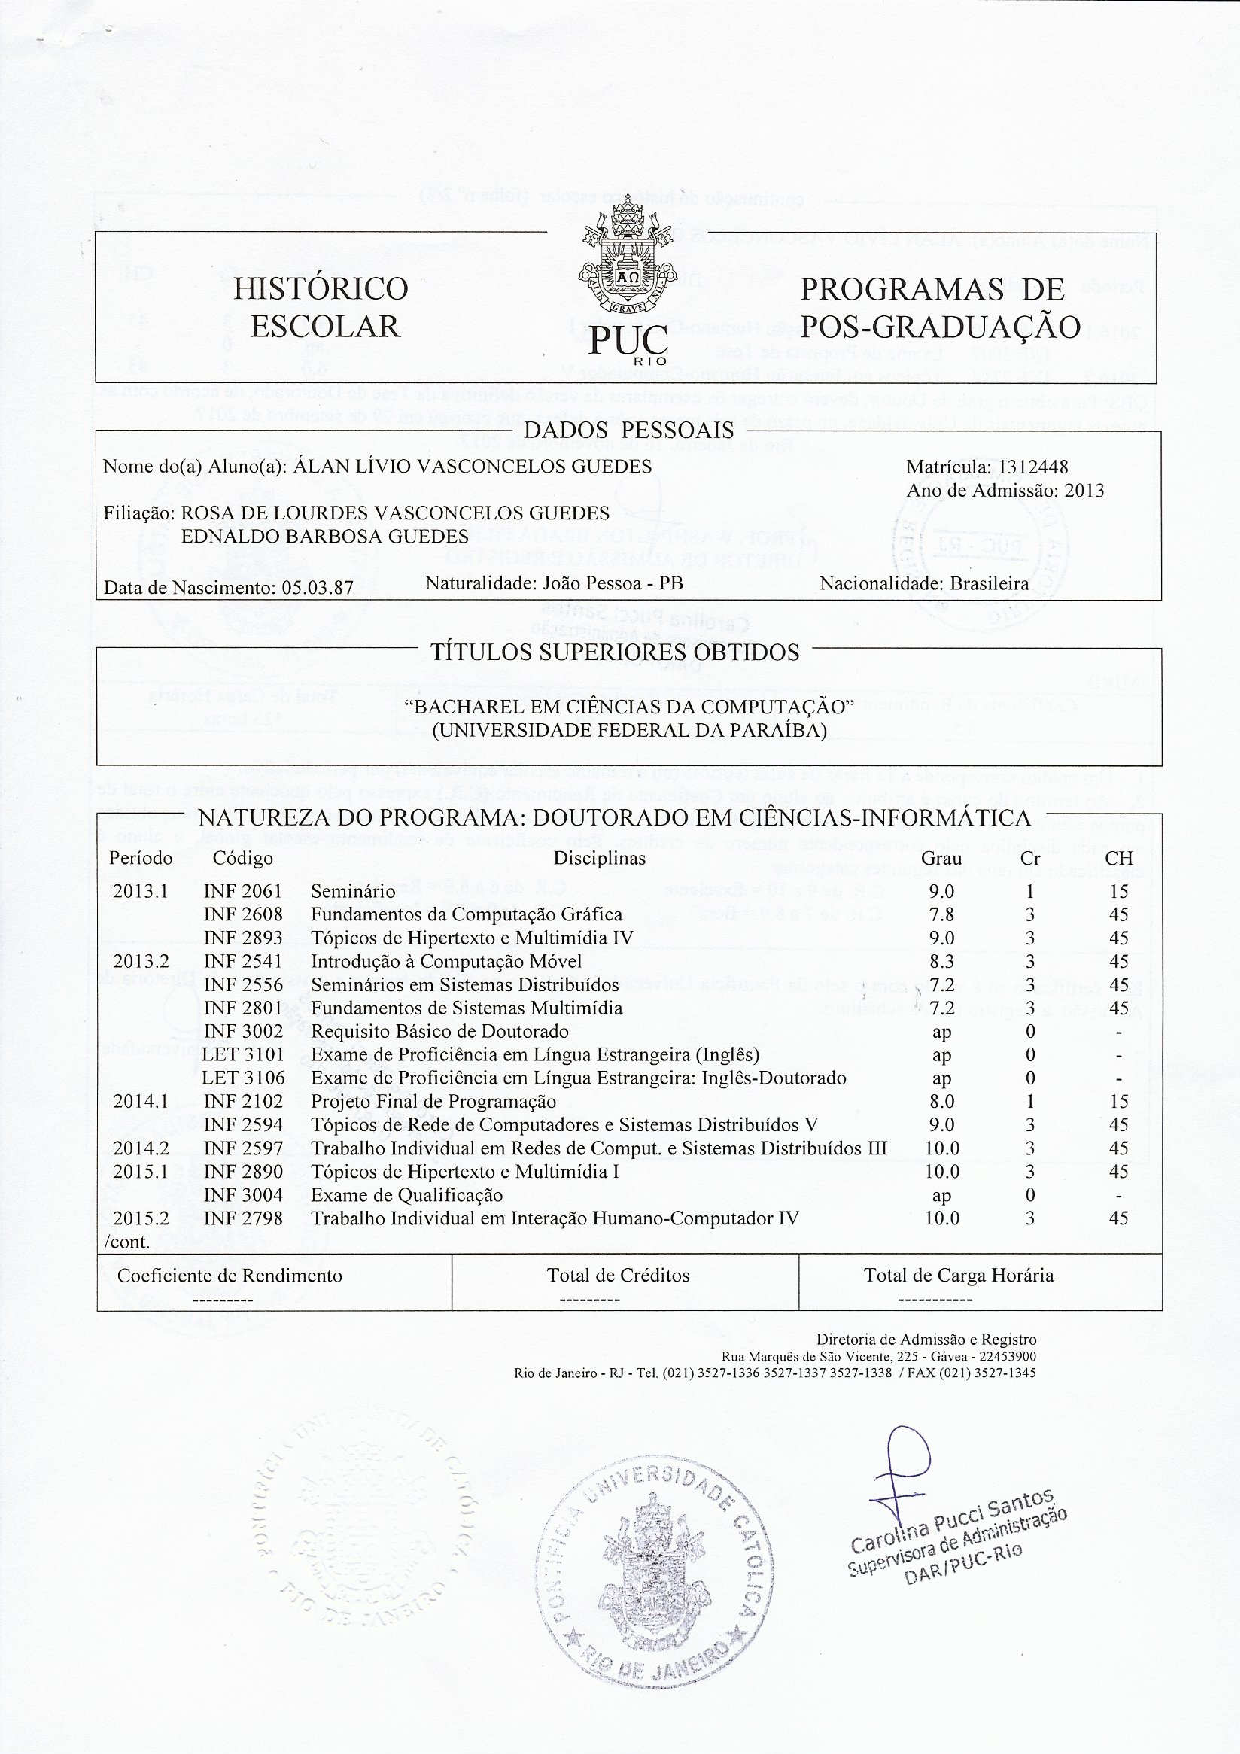
\includegraphics[align=t,width=\textwidth,height=0.6\paperheight, keepaspectratio=true]{certificates/phd-grades.pdf}
\end{figure}

\newpage
The next figure presents the second page of grades from my Ph.D. in Portuguese. In particular, it shows the thesis proposal exam as AP (approved).

\begin{figure}
    \centering
    \includegraphics[align=t,page=2,width=\textwidth,height=0.6\paperheight, keepaspectratio=true]{certificates/phd-grades.pdf}
\end{figure}

%%%%%%%%%%%%%%%%%%%%%%%%%%%%%%%%%%%%%%%%
% PUC-Rio Postdoc certificates
%%%%%%%%%%%%%%%%%%%%%%%%%%%%%%%%%%%%%%%%
\newpage
\section{PUC-Rio Postdoc certficates}
The next two figures shows certifices from my postdoc at PUC-Rio between 2017 and 2019.

\begin{figure}
    \centering
    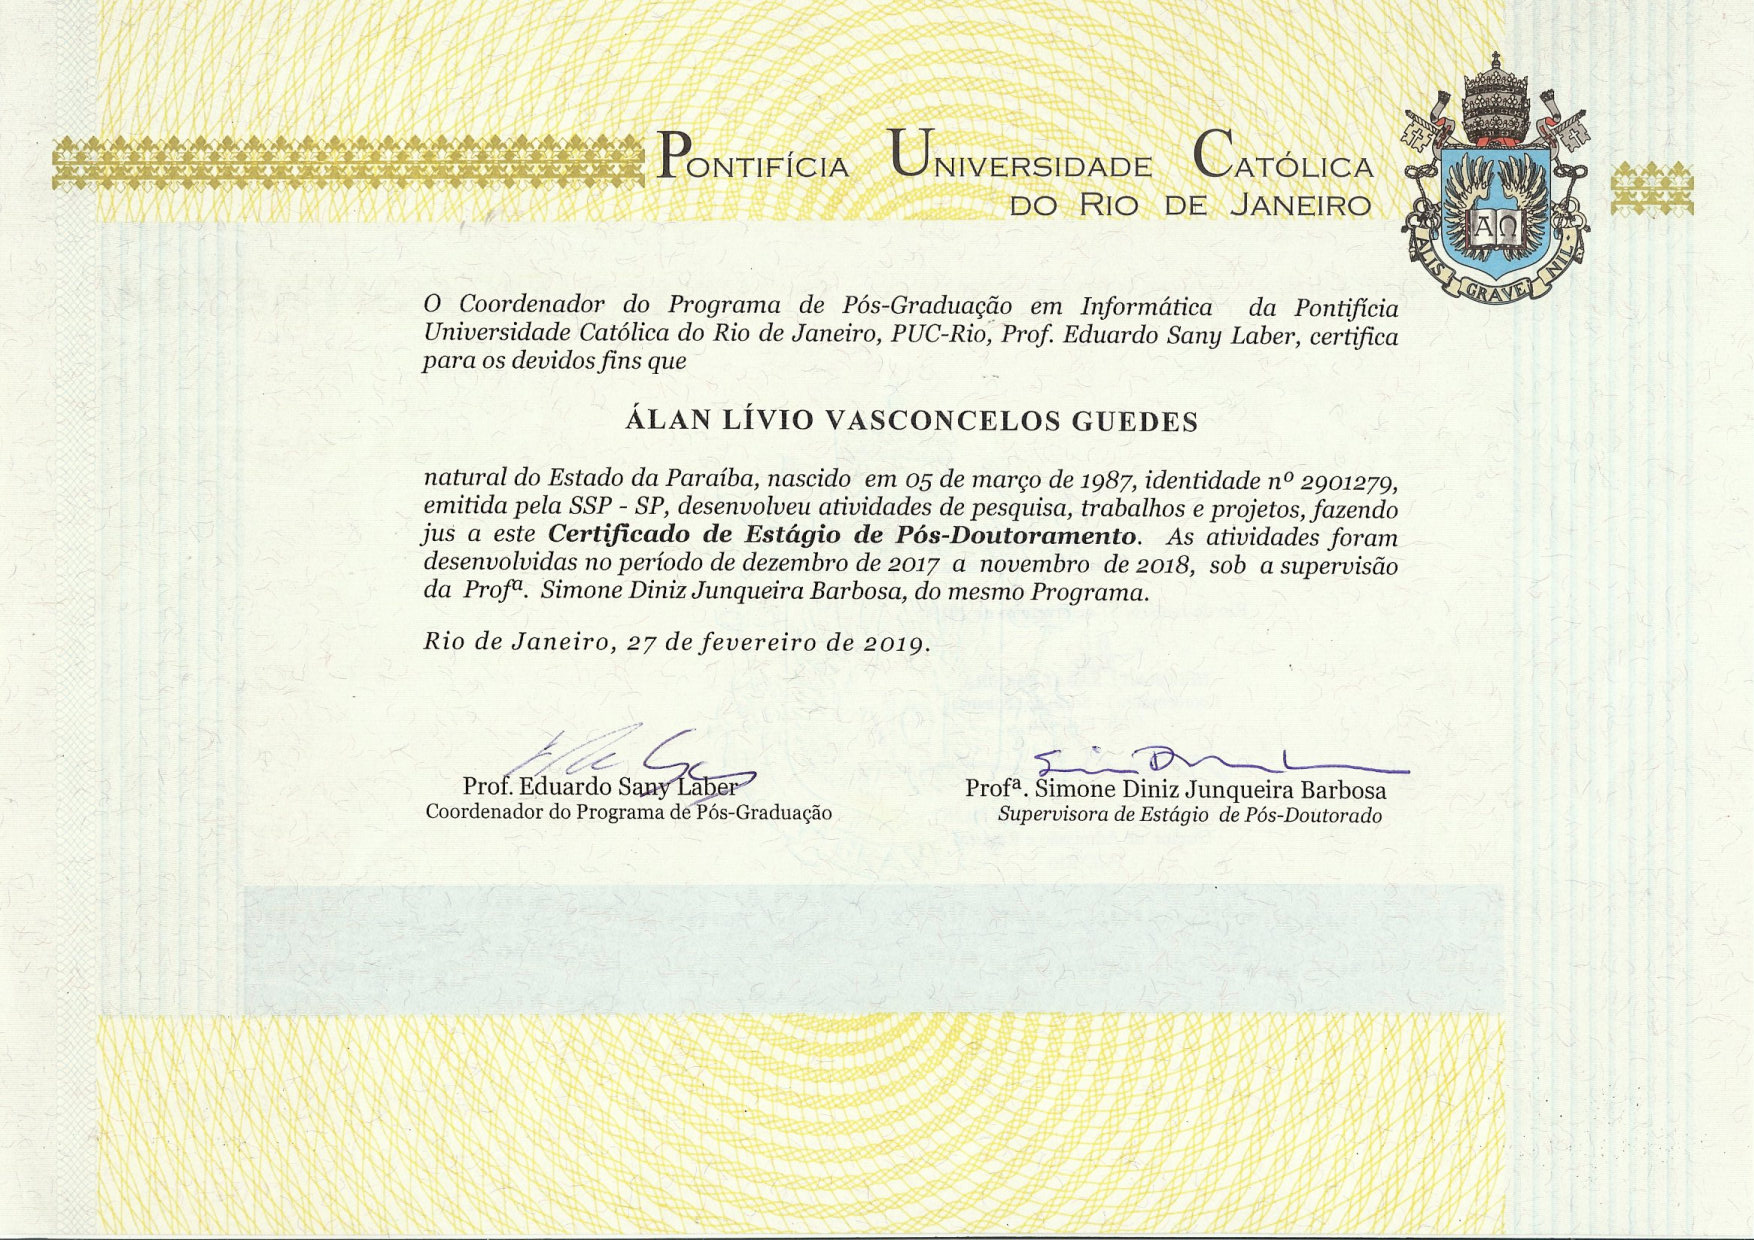
\includegraphics[align=t,width=\textwidth,height=0.3\paperheight, keepaspectratio=true]{certificates/postdoc-pucrio-2017-certificate.pdf}
\end{figure}

\begin{figure}
    \centering
    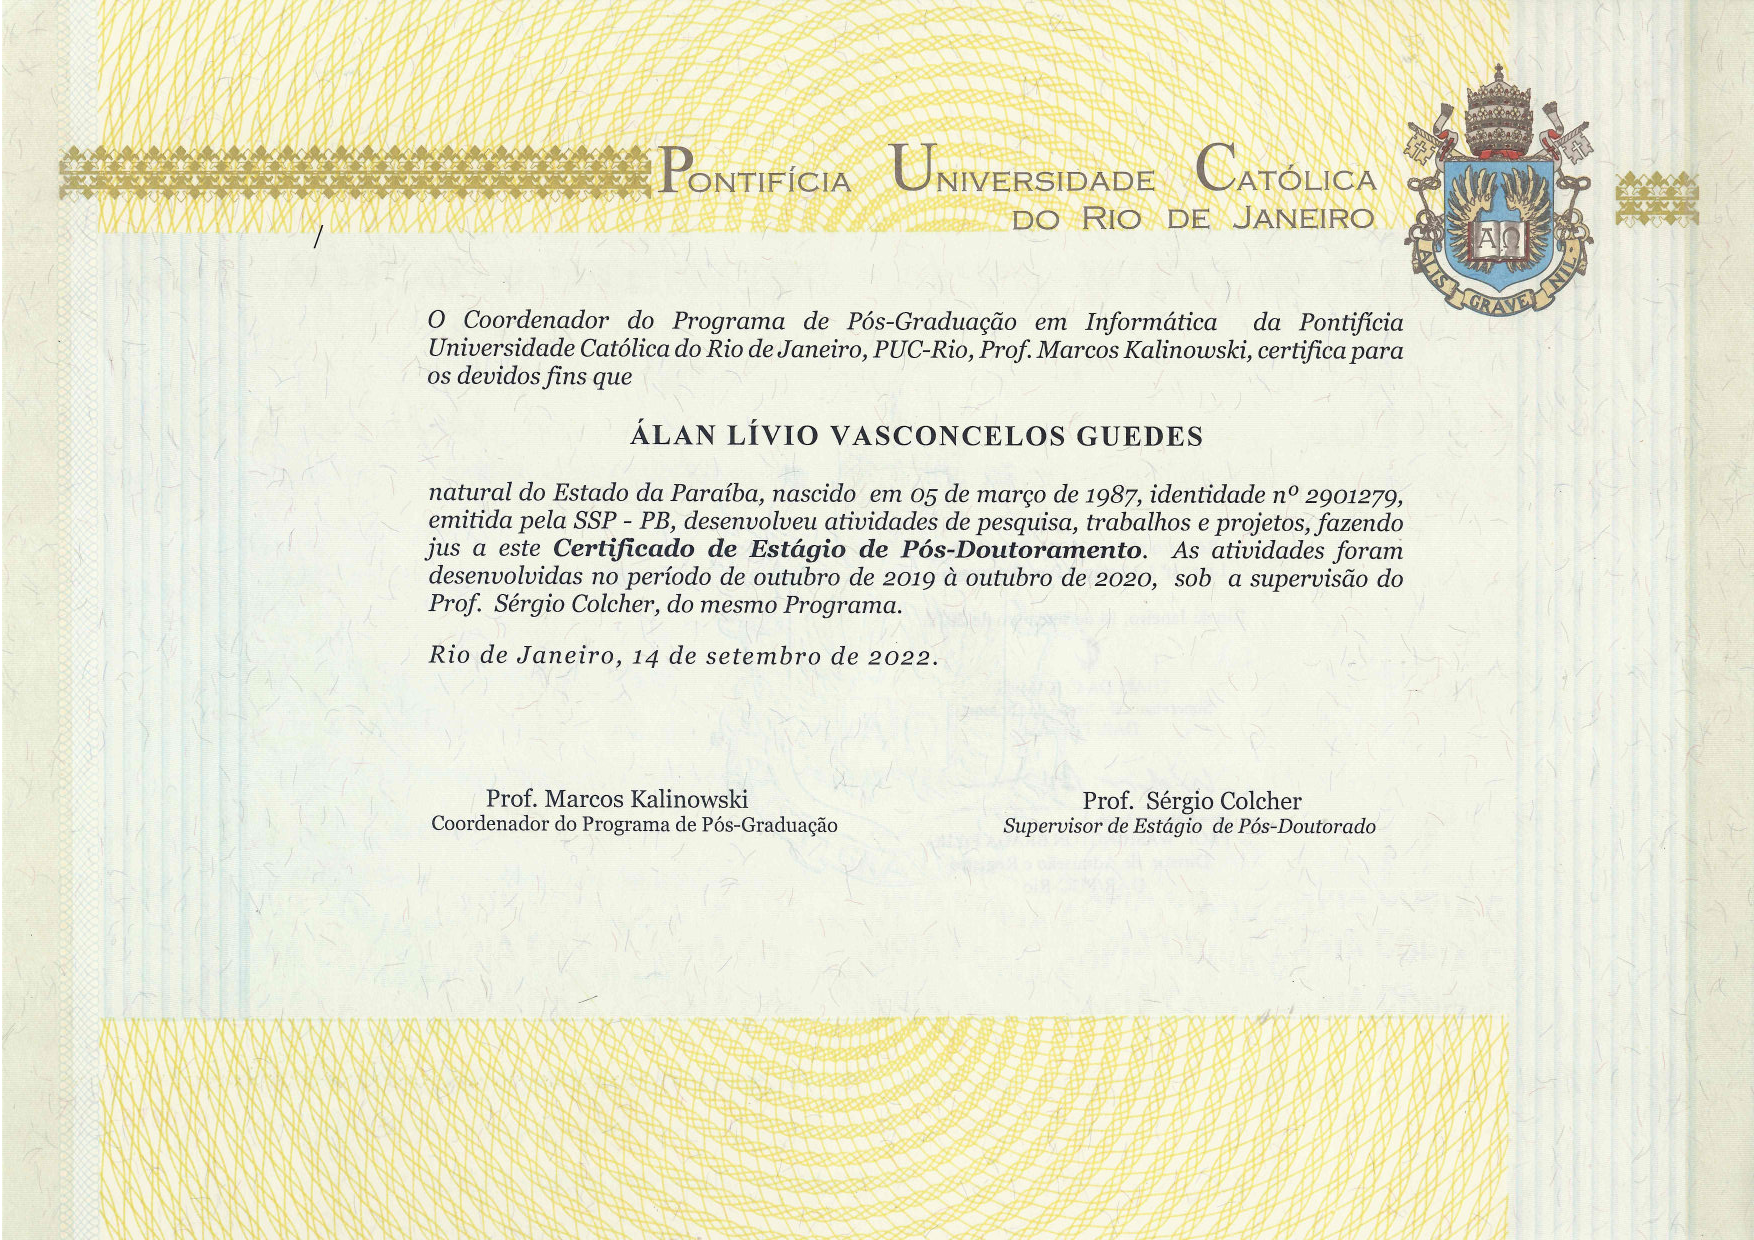
\includegraphics[align=t,width=\textwidth,height=0.3\paperheight, keepaspectratio=true]{certificates/postdoc-pucrio-2018-certificate.pdf}
\end{figure}

%%%%%%%%%%%%%%%%%%%%%%%%%%%%%%%%%%%%%%%%
% UCL postdoc certificate
%%%%%%%%%%%%%%%%%%%%%%%%%%%%%%%%%%%%%%%%
\newpage
\section{UCL Postdoc certficate}
The next two figures shows my certifices from my postdoc at UCL between 2021 and 2023.

\begin{figure}
    \centering
    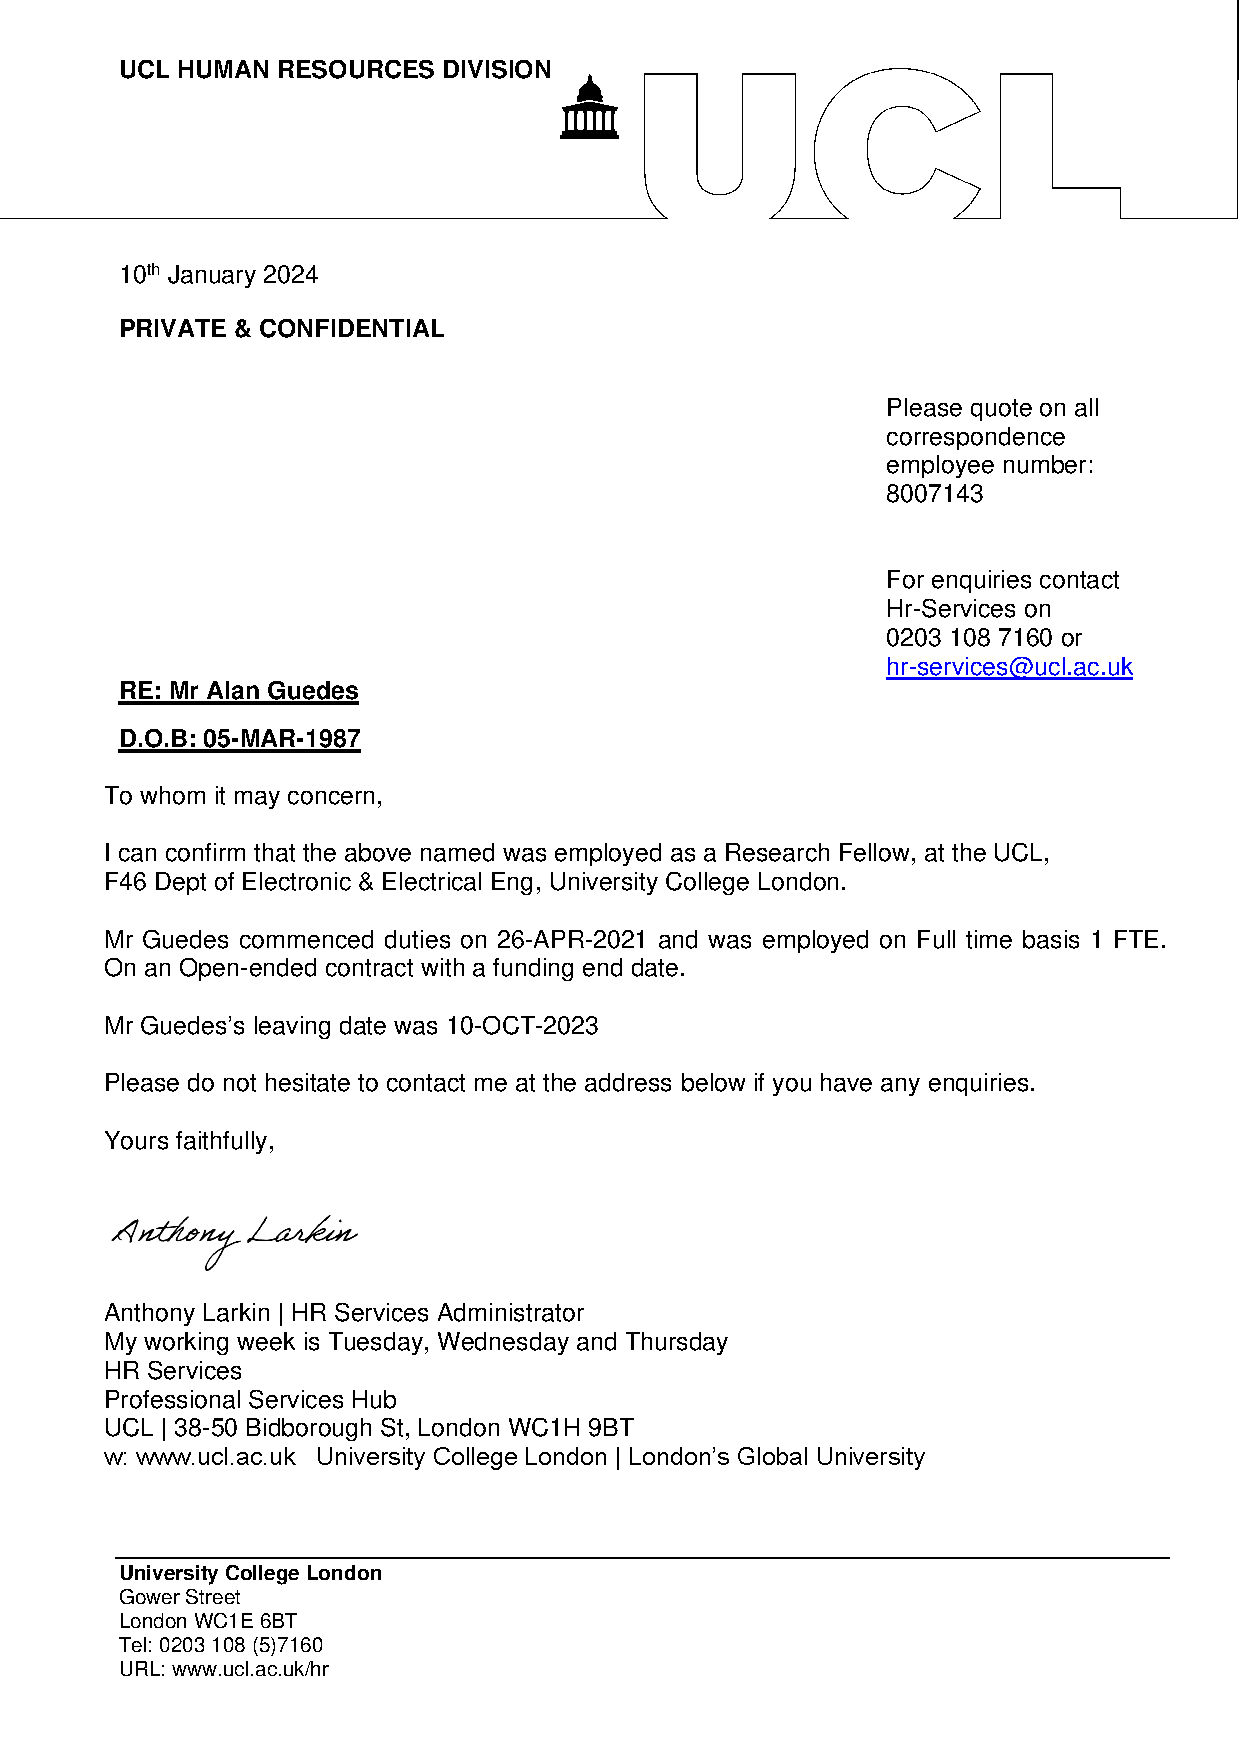
\includegraphics[align=t,width=\textwidth,height=0.6\paperheight, keepaspectratio=true]{certificates/postdoc-ucl-2021-certificate.pdf}
\end{figure}

\section{Academic training certificates}
The next figures present Academic training certificates in topics of Research Supervising, Personal Tutoring, Data protection, People Management, Diversity, and Research Funding.

\begin{figure}
    \centering 
\includegraphics[align=t,width=\textwidth,height=0.18\paperheight, keepaspectratio=true]{certificates/ucl-training/EDI.pdf}
    \centering 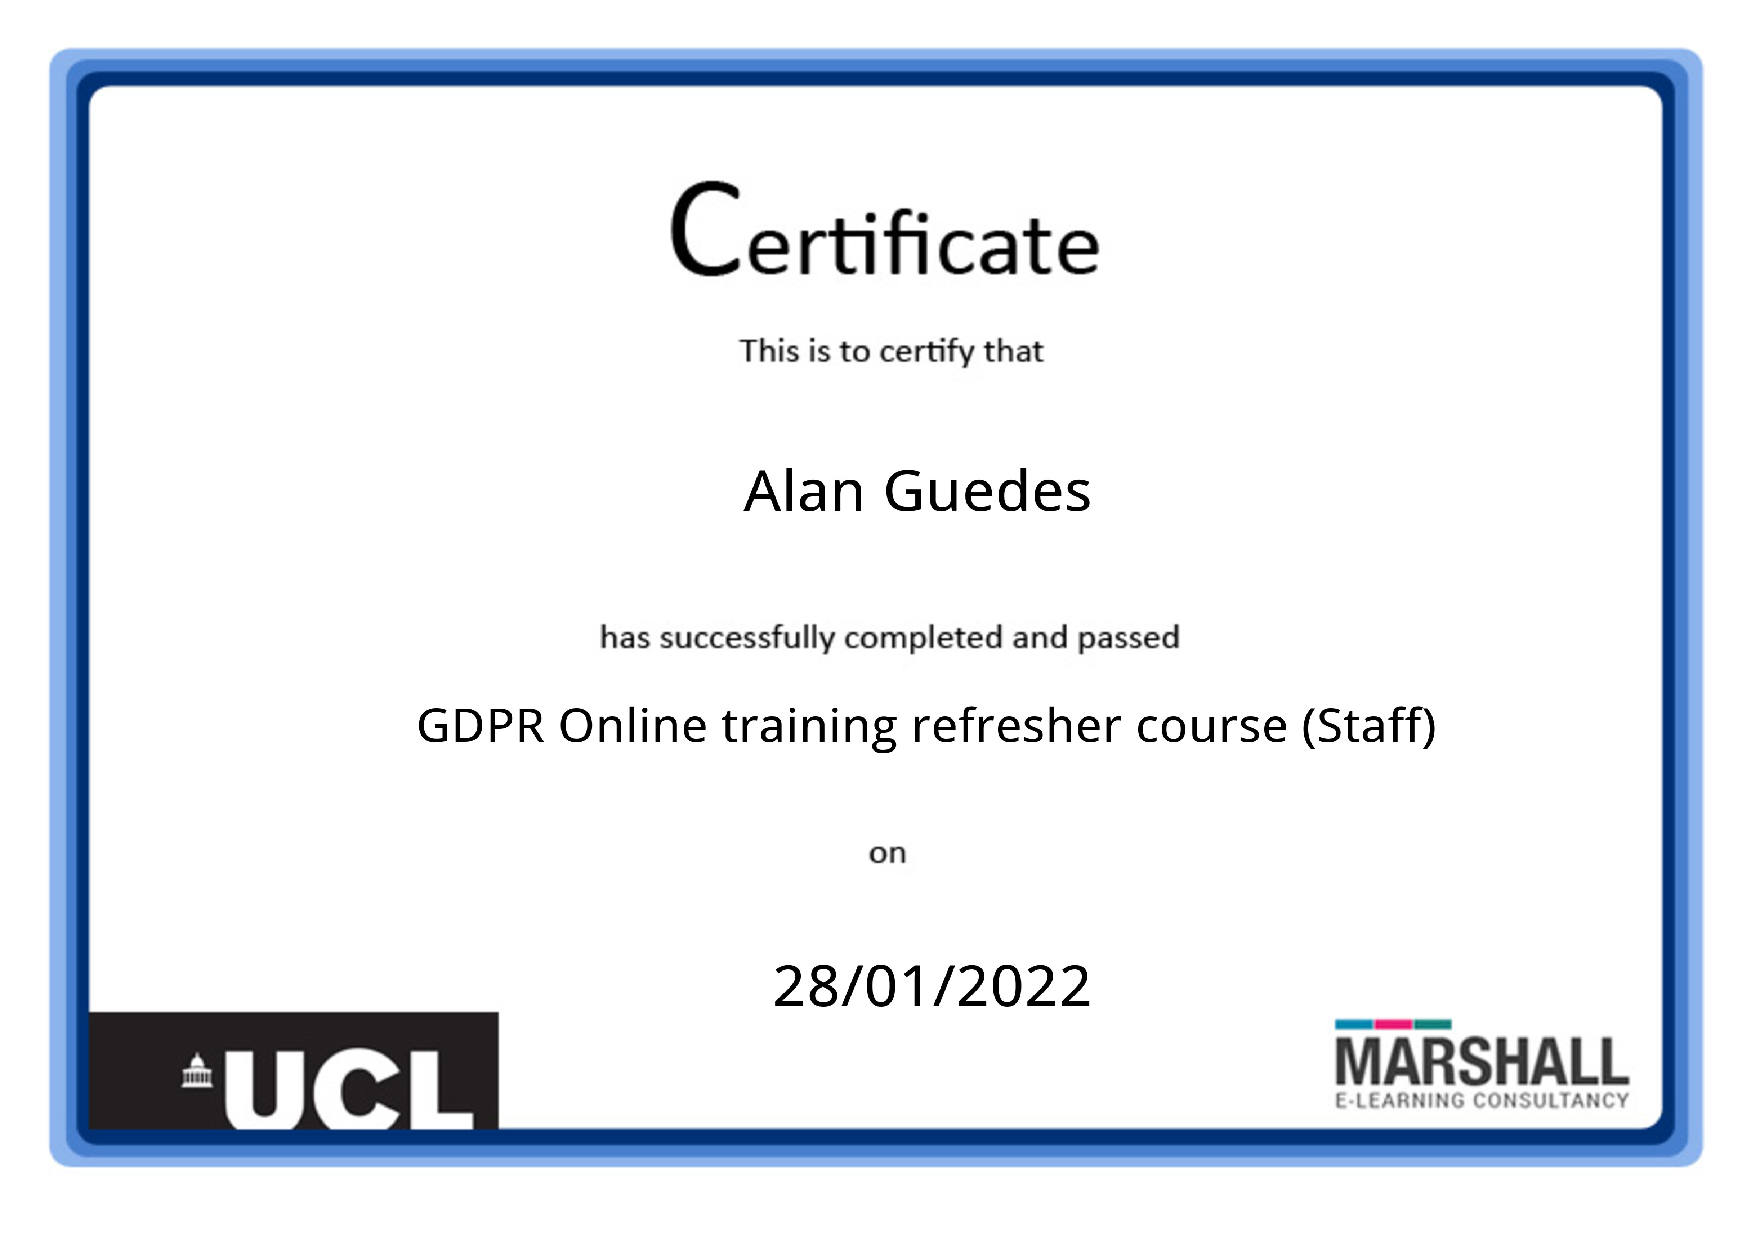
\includegraphics[align=t,width=\textwidth,height=0.18\paperheight, keepaspectratio=true]{certificates/ucl-training/GDPR.pdf}
    \centering 
\includegraphics[align=t,width=\textwidth,height=0.18\paperheight, keepaspectratio=true]{certificates/ucl-training/Data_Protection_and_Freedom_information.pdf}
    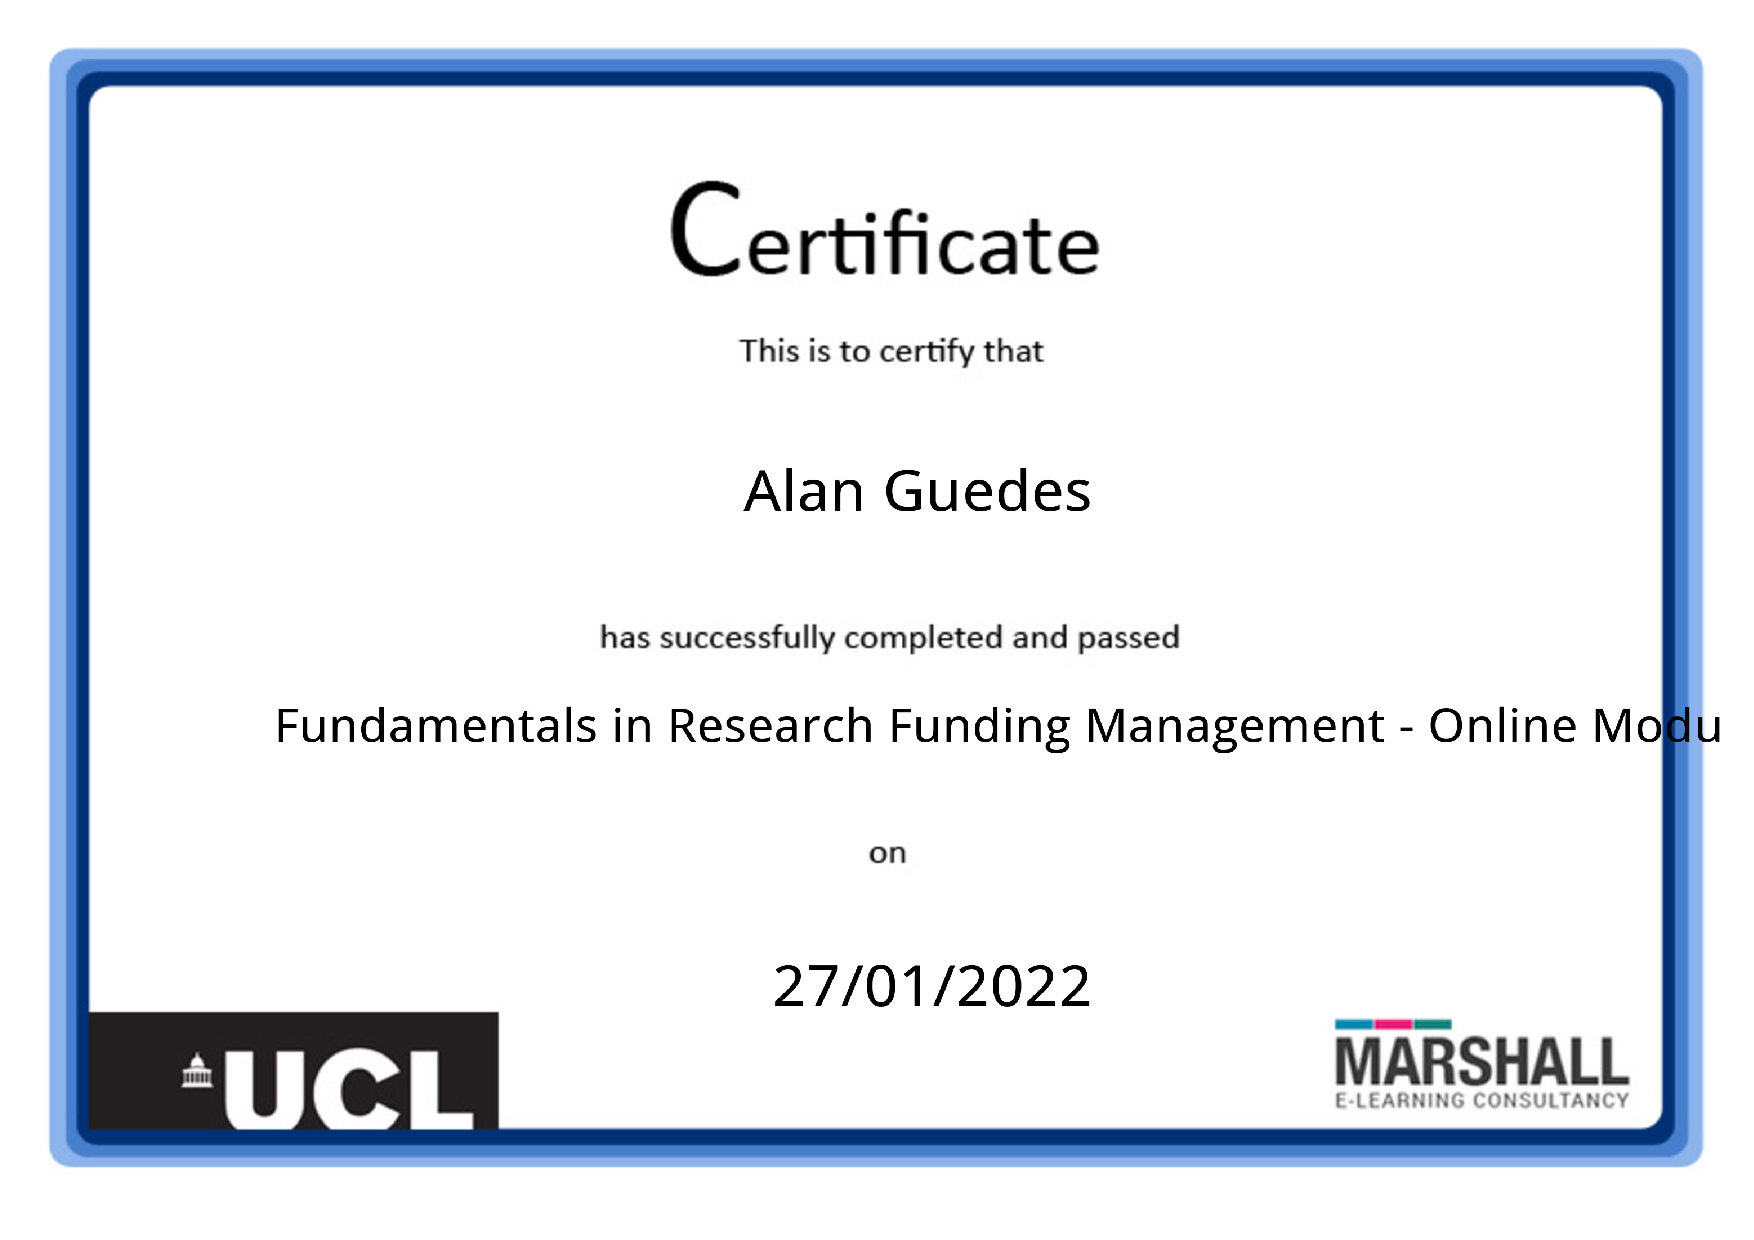
\includegraphics[align=t,width=\textwidth,height=0.18\paperheight, keepaspectratio=true]{certificates/ucl-training/Fundamentals_in_Research_Funding.pdf}
    \centering 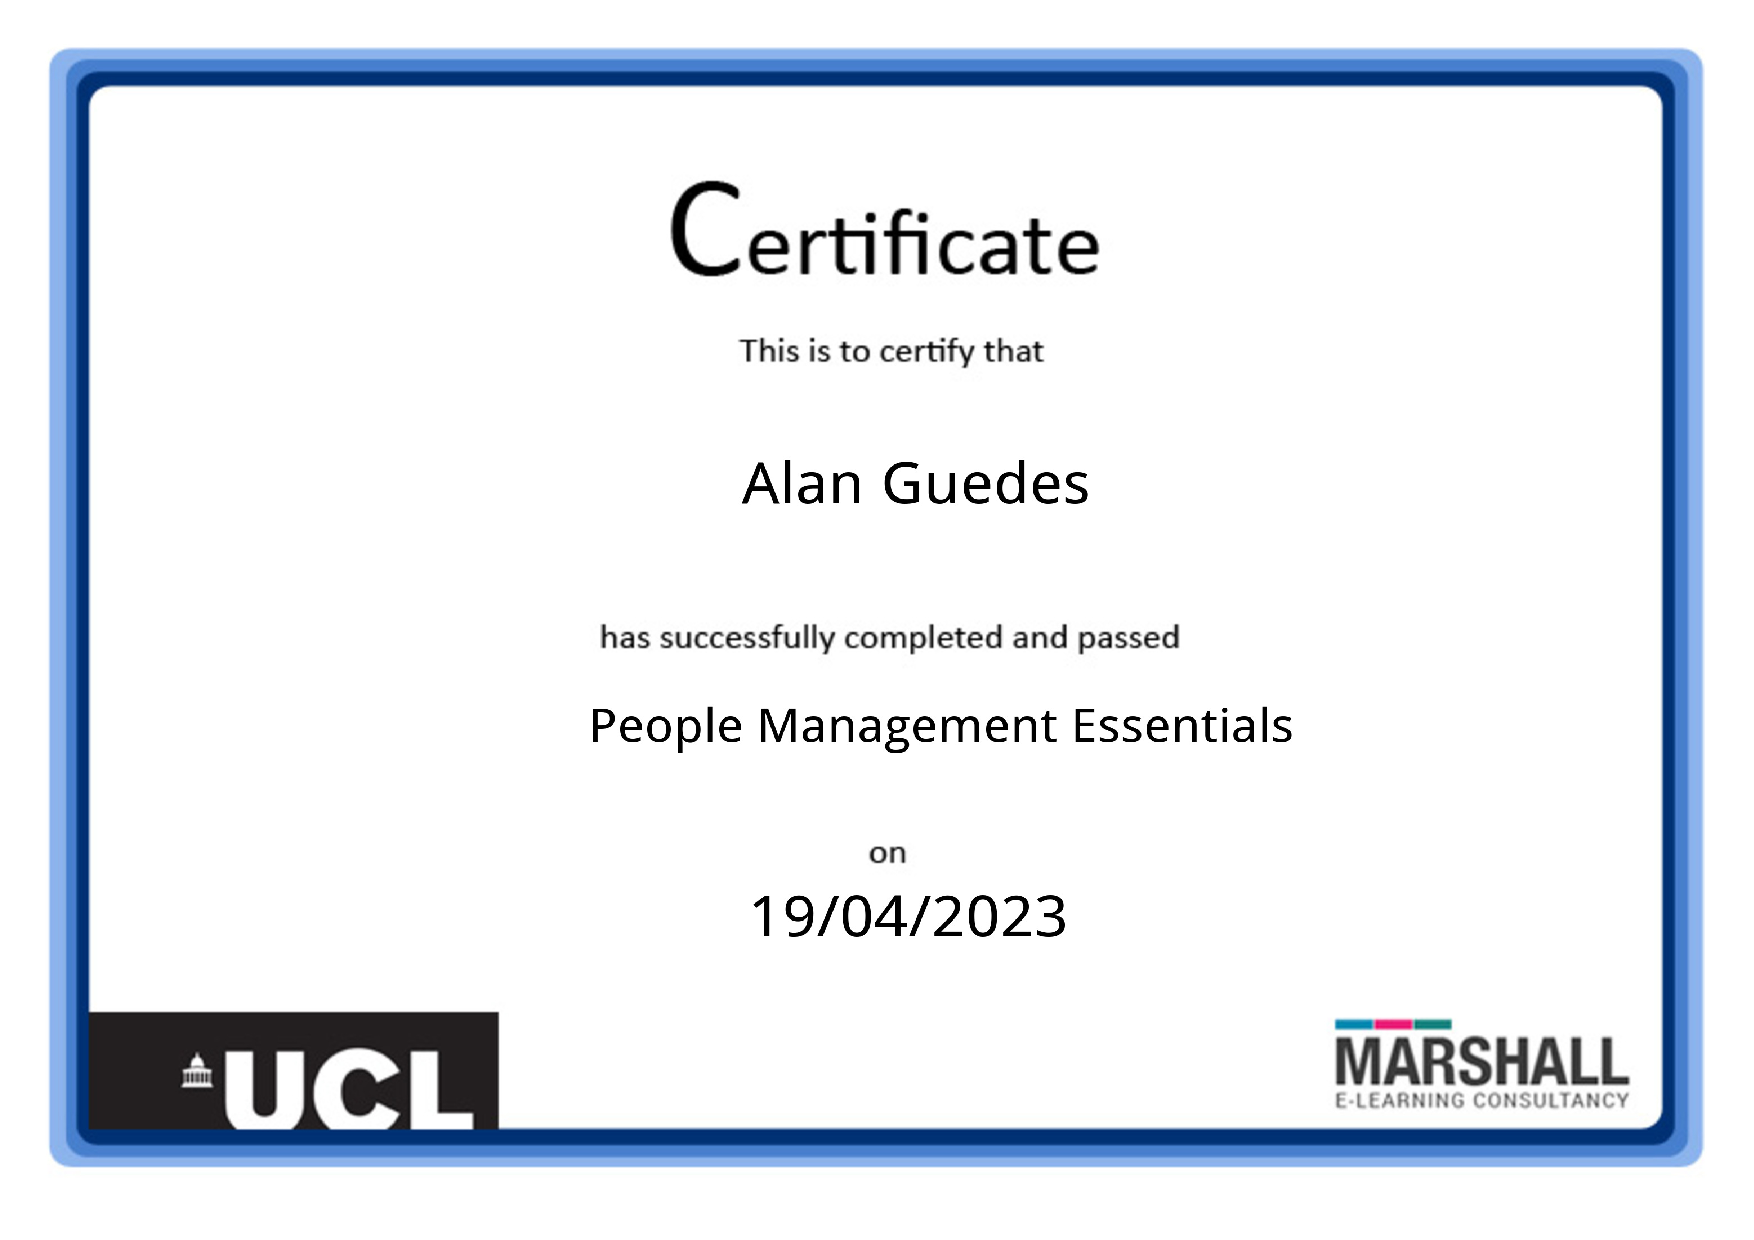
\includegraphics[align=t,width=\textwidth,height=0.18\paperheight, keepaspectratio=true]{certificates/ucl-training/People_Management_Essentials.pdf}
    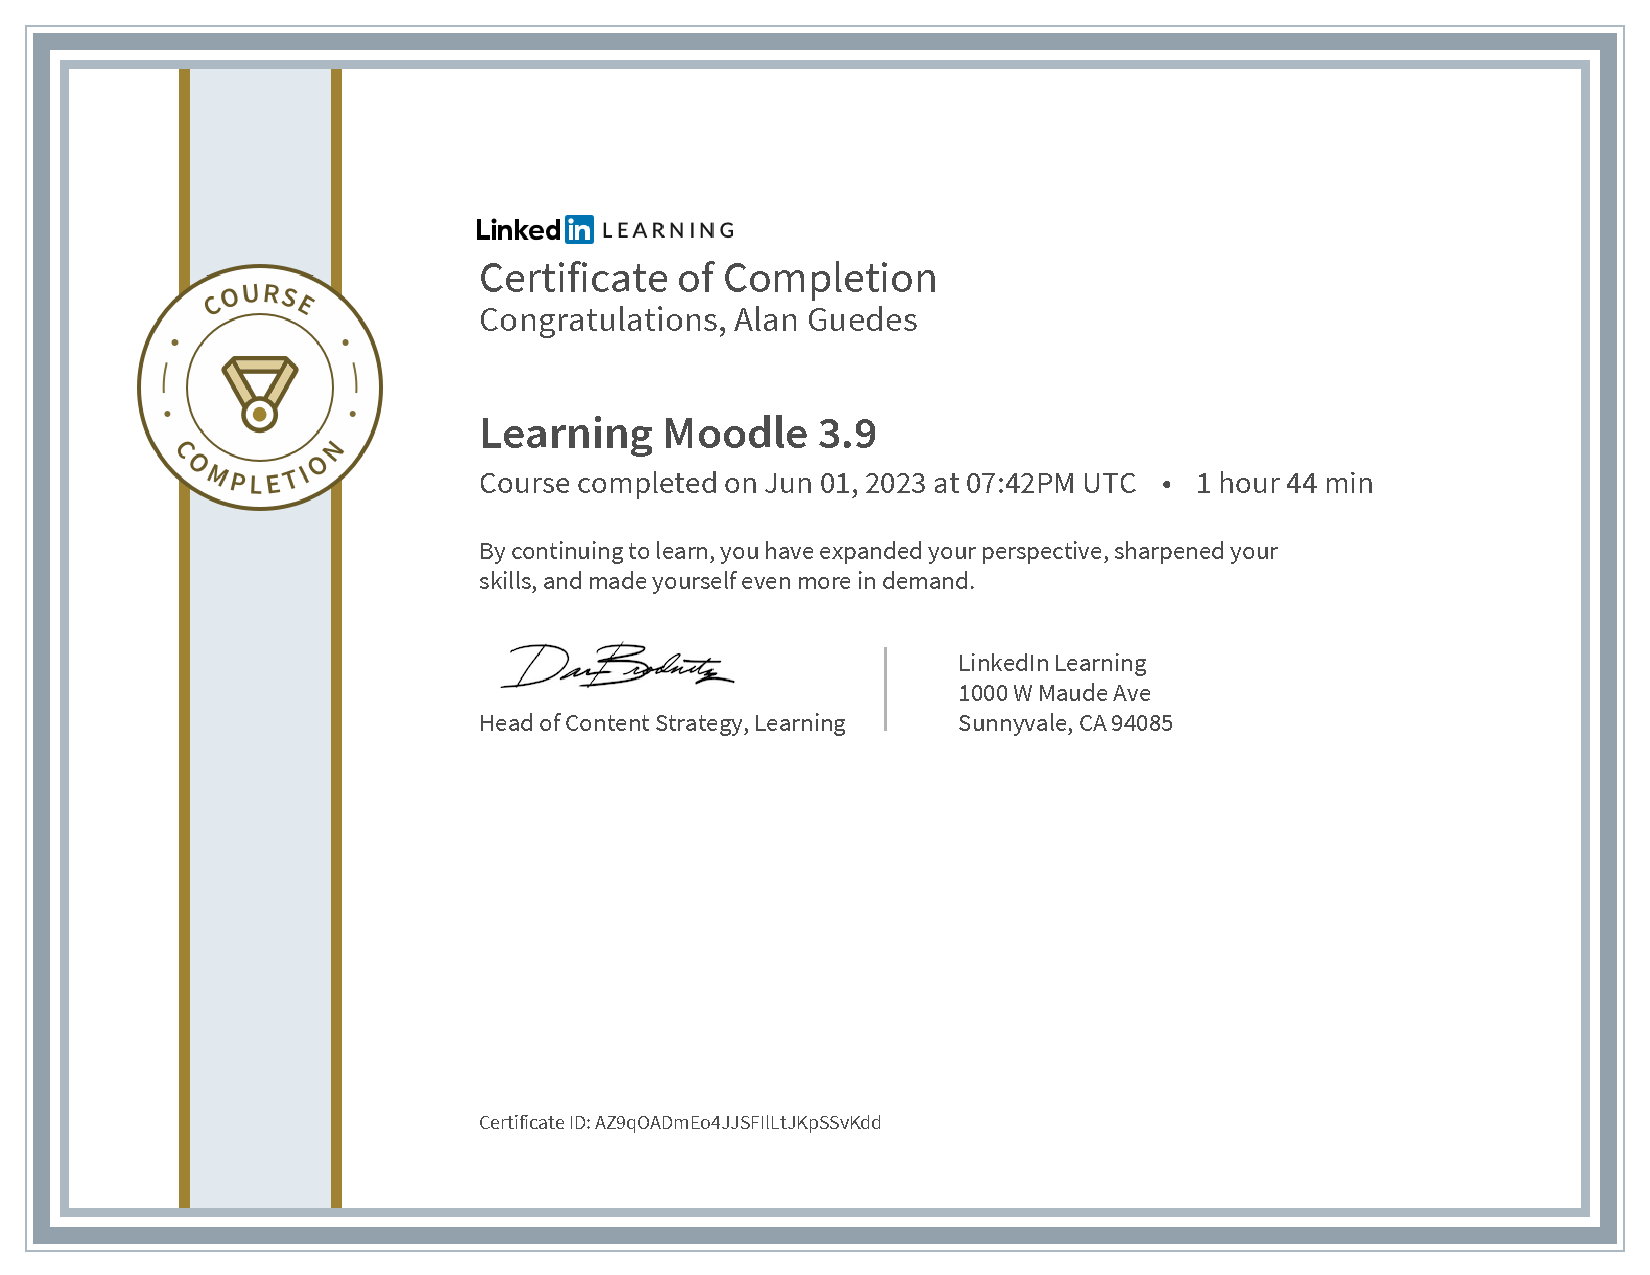
\includegraphics[align=t,width=\textwidth,height=0.18\paperheight, keepaspectratio=true]{certificates/ucl-training/Moodle39.pdf}
\end{figure}
\begin{figure}
    \centering
    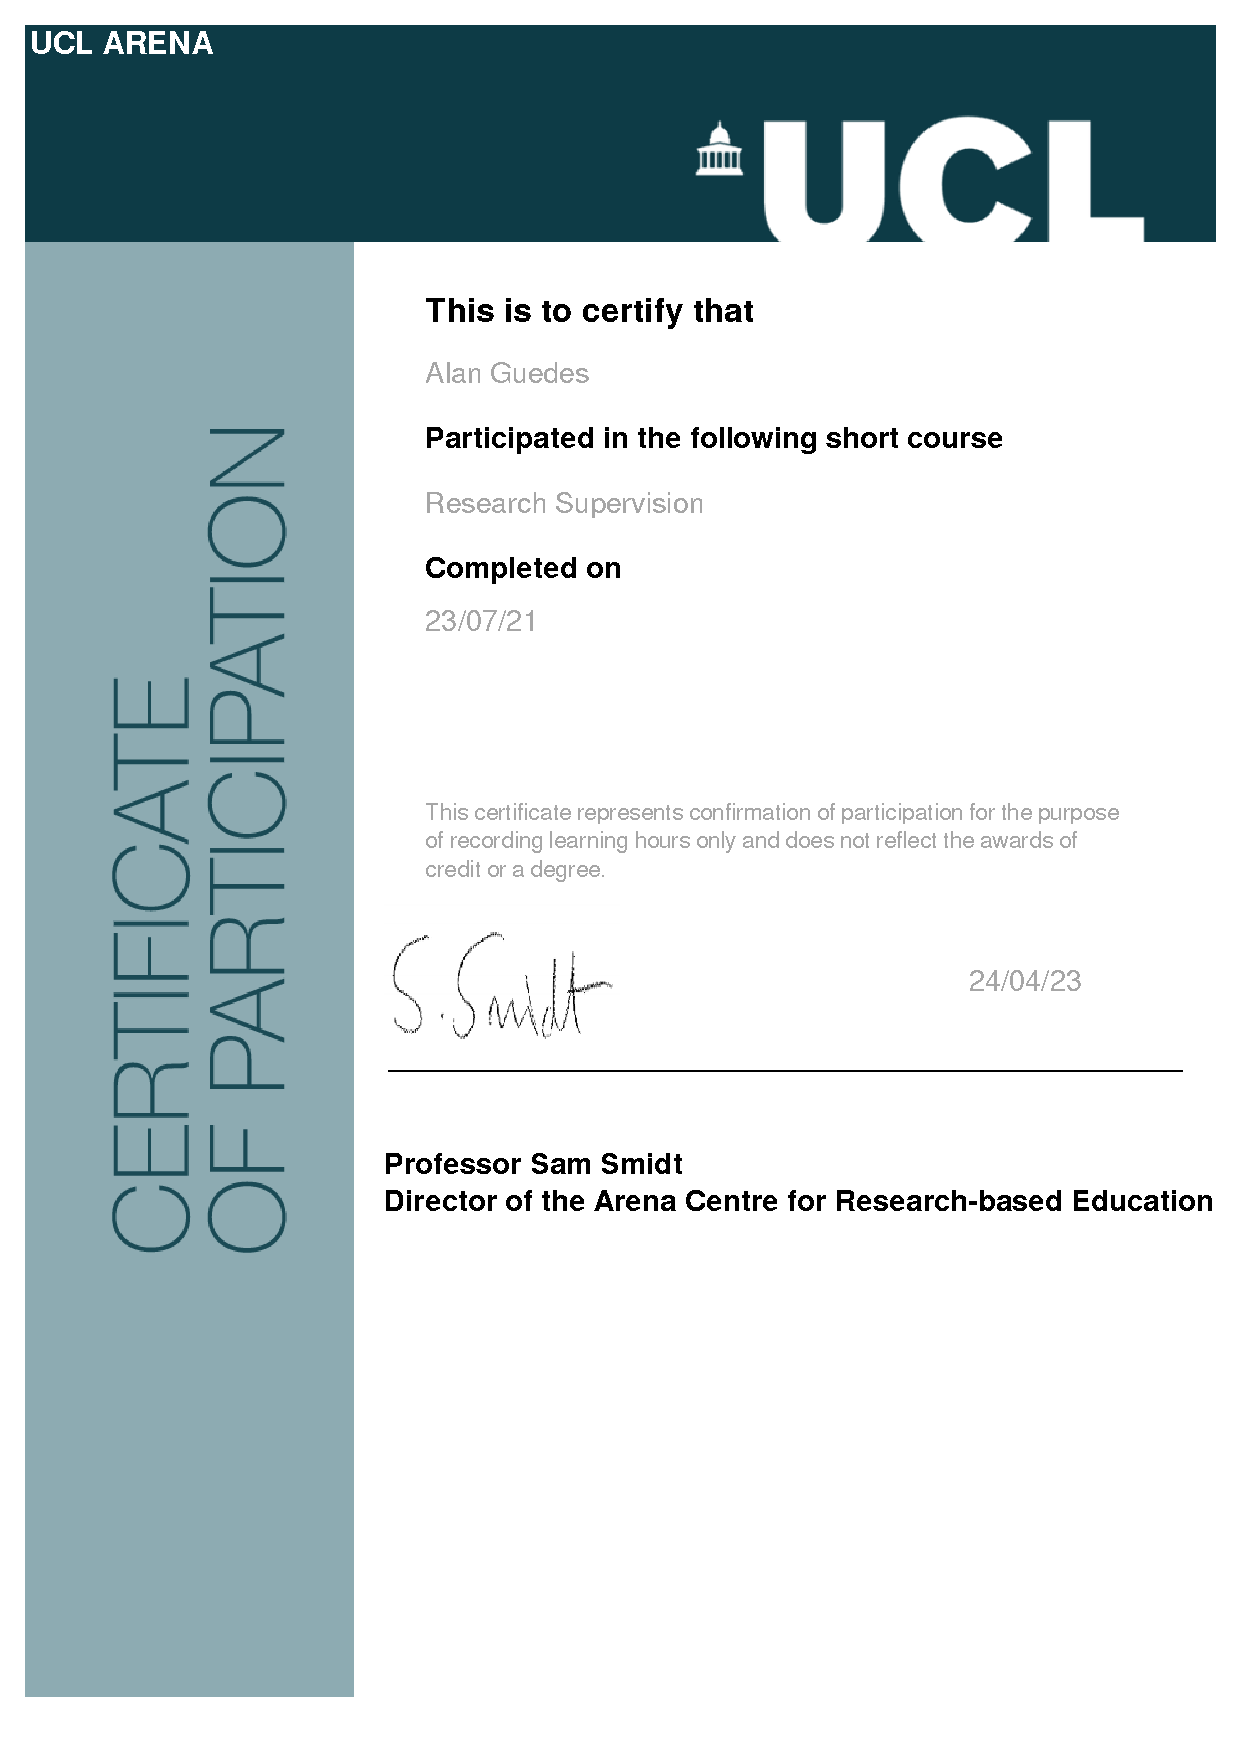
\includegraphics[align=t,width=\textwidth,height=0.3\paperheight, keepaspectratio=true]{certificates/ucl-training/Research_Supervision.pdf}
    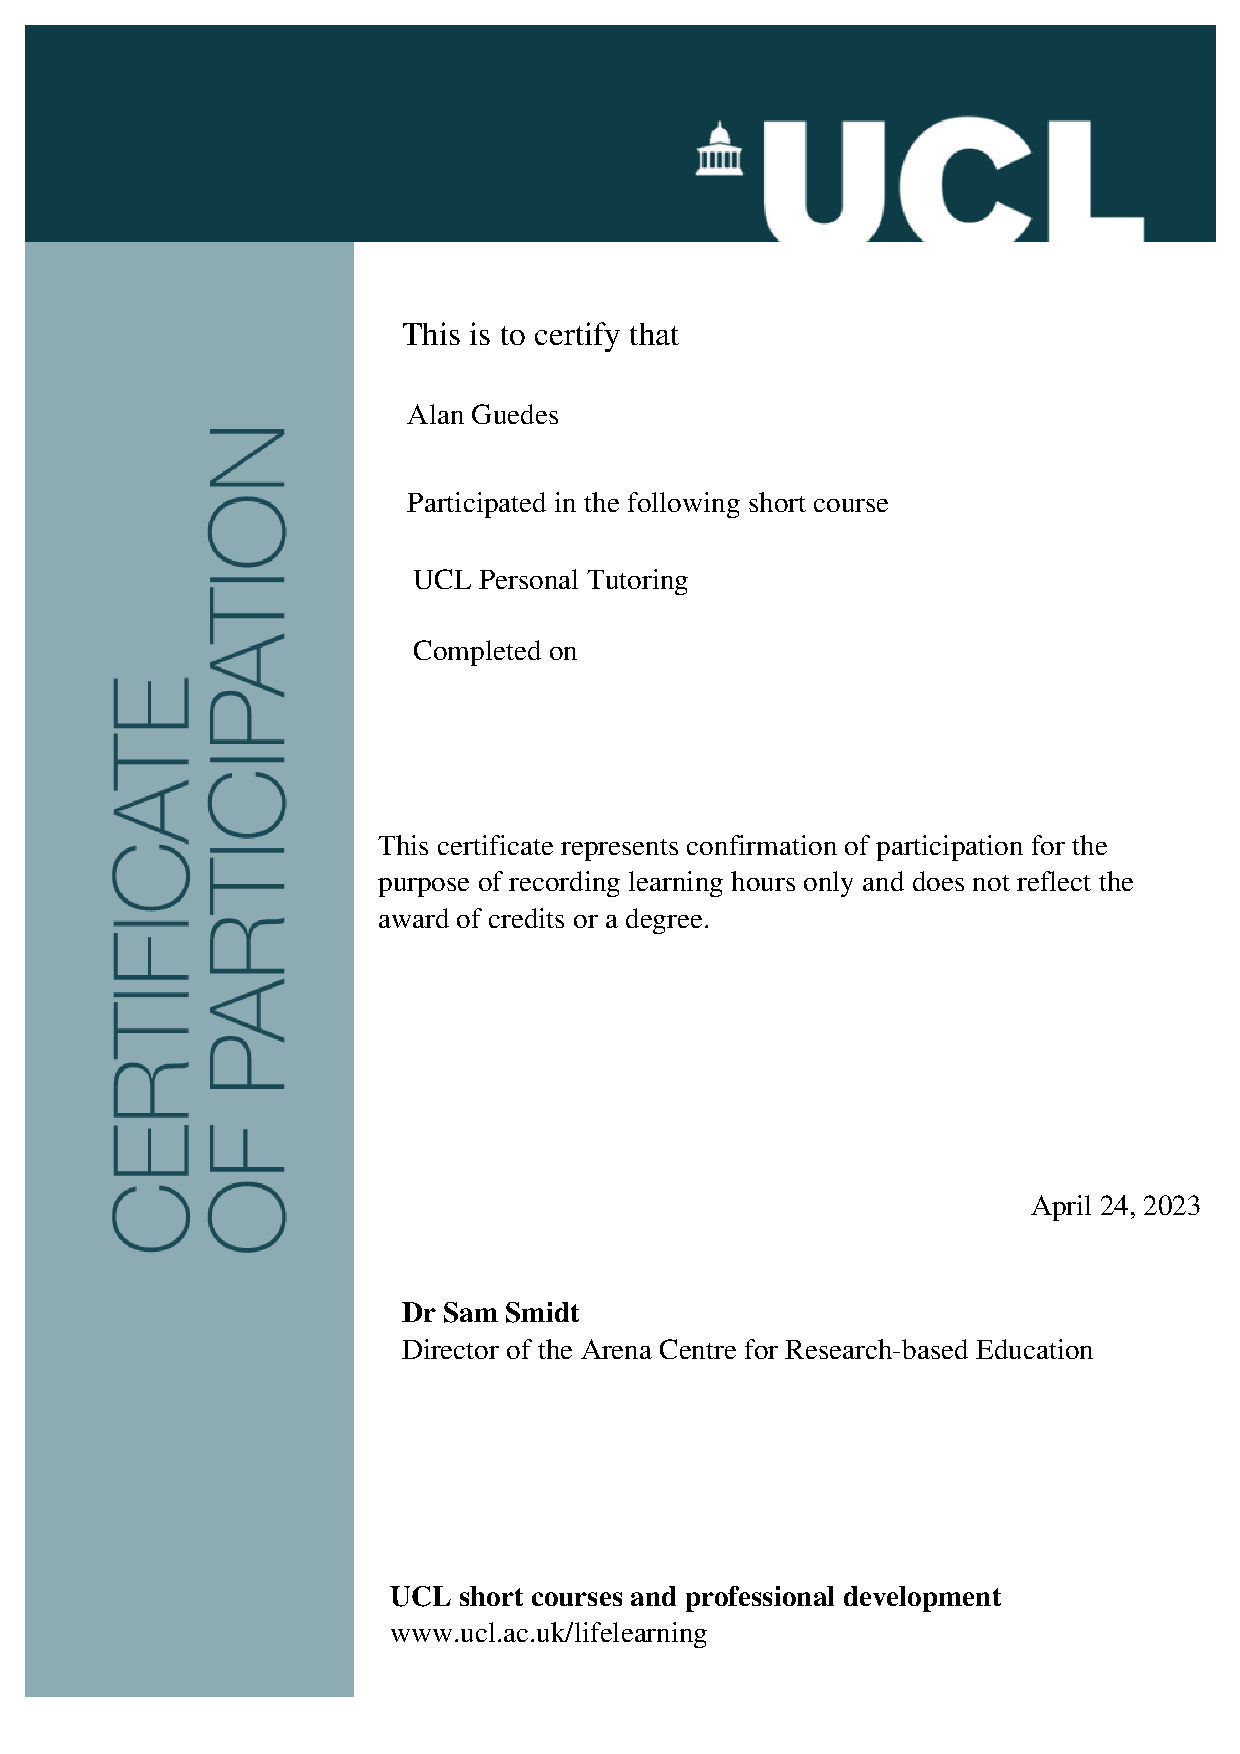
\includegraphics[align=t,width=\textwidth,height=0.3\paperheight, keepaspectratio=true]{certificates/ucl-training/Personal_Tutoring.pdf}
    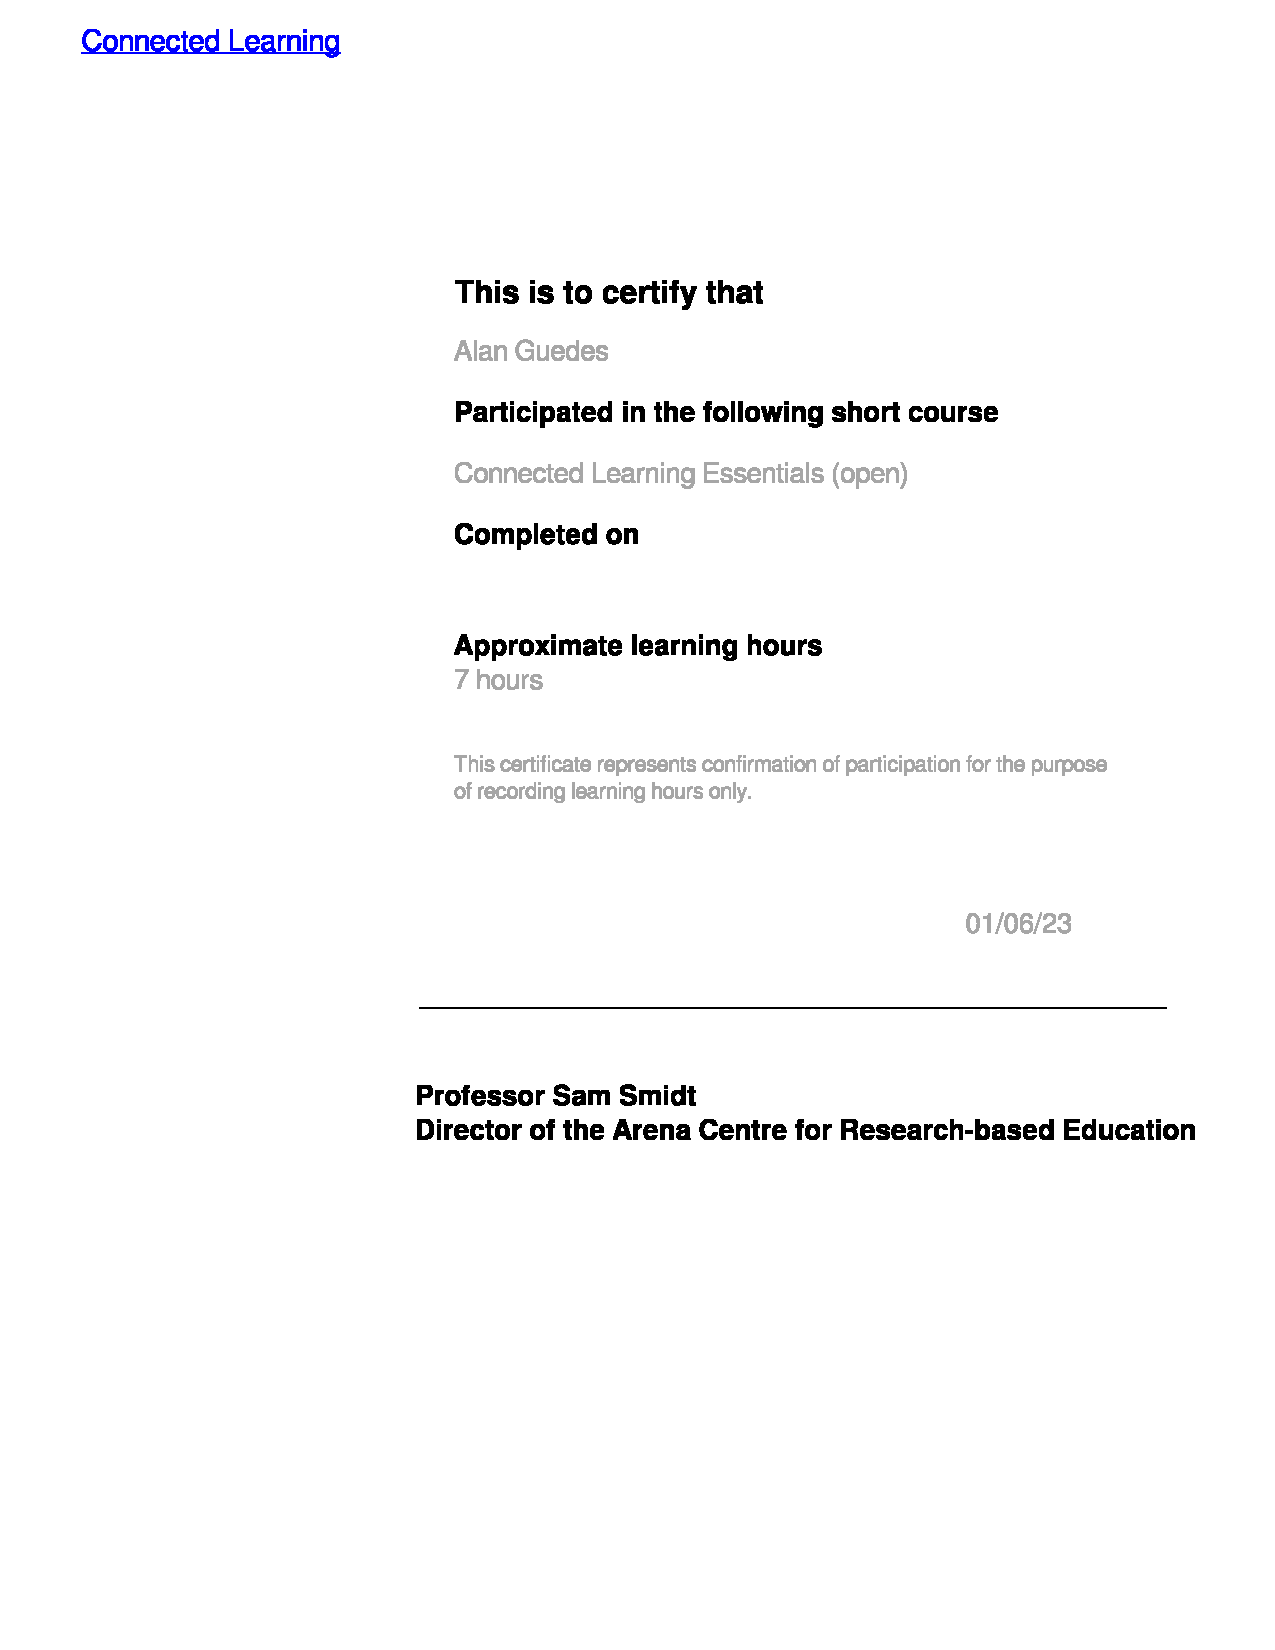
\includegraphics[align=t,width=\textwidth,height=0.5\paperheight, keepaspectratio=true]{certificates/ucl-training/ConnectedLearningEssentials.pdf}
\end{figure}

\begin{figure}
    \centering
    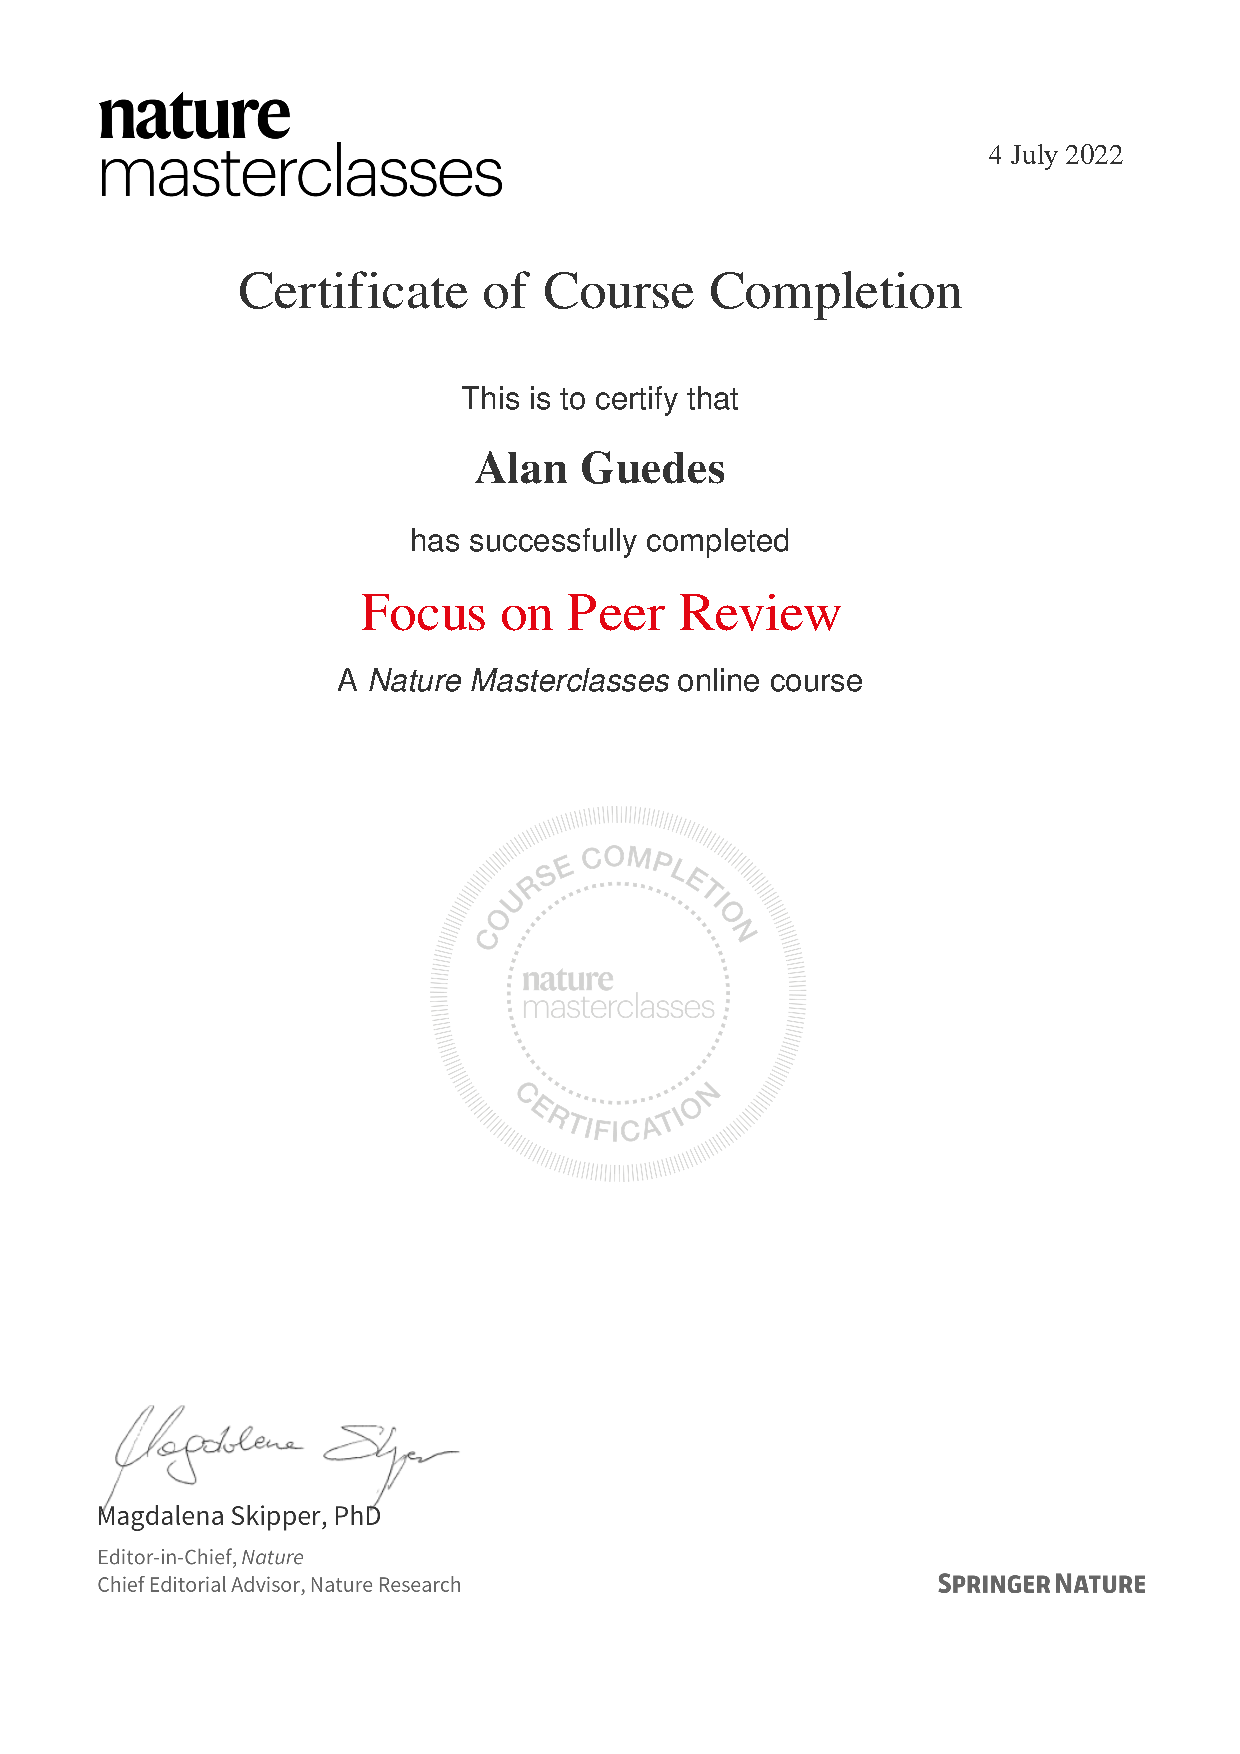
\includegraphics[align=t,width=\textwidth,height=0.4\paperheight, keepaspectratio=true]{certificates/ucl-training/Focus_on_Peer_Review.pdf}
    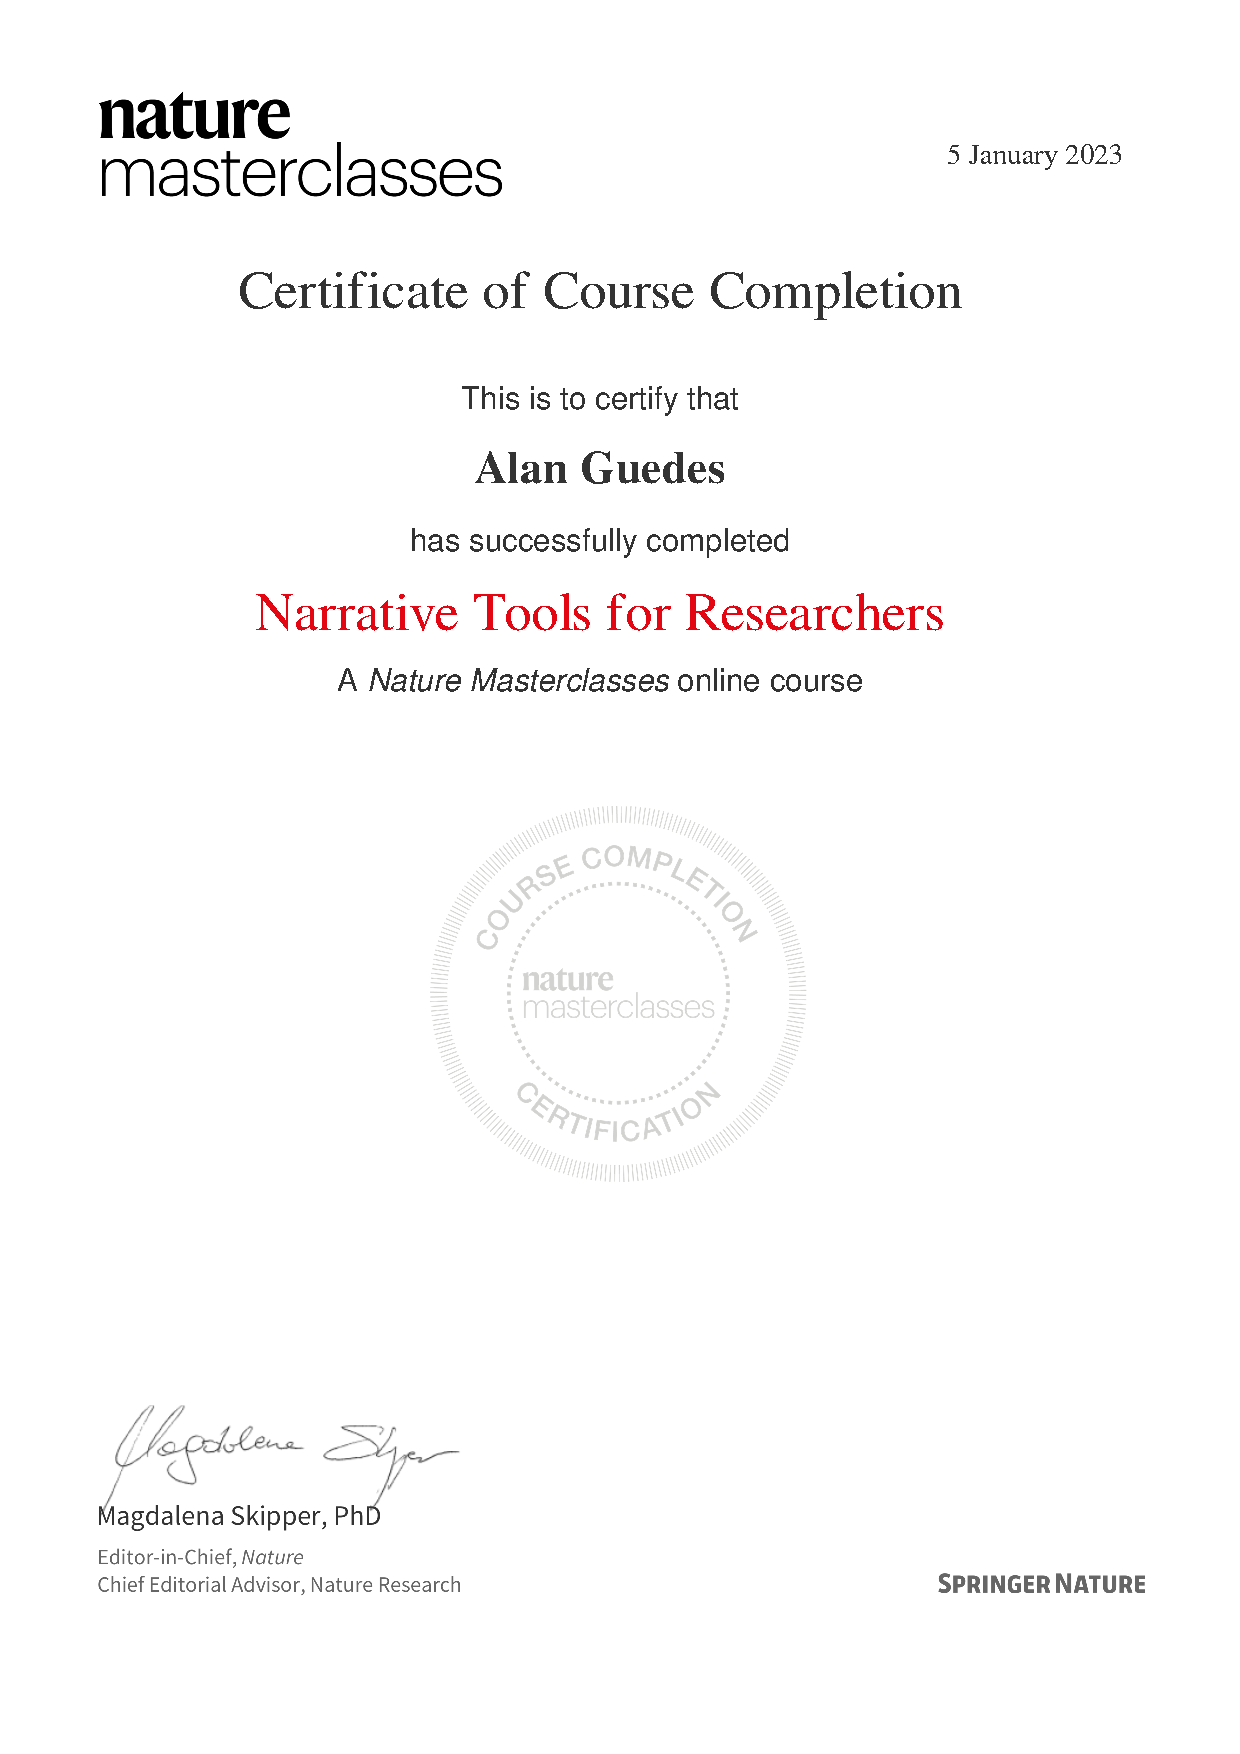
\includegraphics[align=t,width=\textwidth,height=0.4\paperheight, keepaspectratio=true]{certificates/ucl-training/Narrative_Tools_for_Researchers.pdf}
\end{figure}

\end{document}